% ---------------------------------------------------------------------
% --- Arquivo principal e os demais serao os dos capitulos.
% --- EXPRESS�ES ENTRE <> DEVER�O SER COMPLETADAS COM A INFORMA��O ESPEC�FICA DO TRABALHO
% ---------------------------------------------------------------------

\documentclass[ruledheader]{abnt_UFF}

%outline command
\newcount\outlineon
\newcommand{\outline}[1]{\ifnum\outlineon>0\ \\\noindent\fbox{\begin{minipage}{\linewidth}{\footnotesize
#1}\end{minipage}}\\\\\fi}
\newcommand{\exclude}[1]{}

%---pacotes para hiphenizacao e acentuacao em portugues
\usepackage[brazil]{babel}
\usepackage[latin1]{inputenc}
\usepackage[T1]{fontenc}

%--- pacote para melhorar a defini��o das fontes.
\usepackage{lmodern}


%--- pacote para figuras
\usepackage{epsf}
%\usepackage[dvips]{epsfig,graphicx}
\usepackage{epsfig,graphicx}
\usepackage{subfigure}


%--- pacote de simbolos
\usepackage{latexsym}
\usepackage{textcomp}

%--- simbolos matematicos
\usepackage{amsmath}
\usepackage{amssymb}

%--- pacote para gerar pseudo-codigo
\usepackage{algorithm}
\usepackage{algorithmic}
\floatname{algorithm}{Algoritmo}
\usepackage{verbatim}
\usepackage{float, fancyvrb}

%--- outros pacotes
\usepackage{url}
\usepackage{longtable}
\usepackage{lscape}


%Tabela Colorida
\usepackage{colortbl}


\usepackage{multicol}
\usepackage{multirow}
\usepackage{rotating}

% Add cor na table // HDS
\usepackage[table]{xcolor}  

\hyphenation{
a-de-qua-da-men-te
di-men-sio-na-men-to
}

%---------usando tipo de fonte padrao
\renewcommand{\ABNTchapterfont}{\bfseries\fontfamily{cmr}\fontseries{b}\selectfont}
\renewcommand{\ABNTsectionfont}{\bfseries\fontfamily{cmr}}


% --- -----------------------------------------------------------------
% --- Documento Principal.
% --- -----------------------------------------------------------------
% \usepackage[pdftex]{hyperref}
% \hypersetup{colorlinks, sitecolor=black, pdftex}
\begin{document}

% --- -----------------------------------------------------------------
% --- Titulo, abstract, dedicatorias e agradecimentos.
% --- Indice geral, lista de figuras e tabelas.
% --- -----------------------------------------------------------------
% --- -----------------------------------------------------------------
% --- Elementos usados na Capa e na Folha de Rosto.
% --- EXPRESS�ES ENTRE <> DEVER�O SER COMPLETADAS COM A INFORMA��O ESPEC�FICA DO TRABALHO
% --- E OS S�MBOLOS <> DEVEM SER RETIRADOS 
% --- -----------------------------------------------------------------
\autor{HEDER DORNELES SOARES} % deve ser escrito em maiusculo

\titulo{SINCRONIZA��O EM REDES SENSORES SEM FIO}

\instituicao{UNIVERSIDADE FEDERAL FLUMINENSE}

\orientador{C�LIO VINICIUS NEVES DE ALBUQUERQUE}

\coorientador{RAPHAEL PEREIRA DE OLIVEIRA GUERRA} % se nao existir co-orientador apague essa linha

\local{NITER\'{O}I}

\data{2016} % ano da defesa

\comentario{Disserta��o de Mestrado apresentada ao Programa de P\'{o}s-Gradua\c{c}\~{a}o em Computa\c{c}\~{a}o da \mbox{Universidade} Federal Fluminense como requisito parcial para a obten\c{c}\~{a}o do Grau de \mbox{Mestre em Computa\c{c}\~{a}o}. \'{A}rea de concentra\c{c}\~{a}o: \mbox{Redes e Sistemas Distribu�dos e Paralelos}} %preencha com a sua area de concentracao


% --- -----------------------------------------------------------------
% --- Capa. (Capa externa, aquela com as letrinhas douradas)(Obrigatorio)
% --- ----------------------------------------------------------------
\capa

% --- -----------------------------------------------------------------
% --- Folha de rosto. (Obrigatorio)
% --- ----------------------------------------------------------------
\folhaderosto


\pagestyle{ruledheader}
\setcounter{page}{1}
\pagenumbering{roman}

% --- -----------------------------------------------------------------
% --- Termo de aprovacao. (Obrigatorio)
% --- ----------------------------------------------------------------
\cleardoublepage
\thispagestyle{empty}

\vspace{-60mm}

\begin{center}
   {\large HEDER DORNELES SOARES}\\
   \vspace{7mm}

   SINCRONIZA��O EM REDES SENSORES SEM FIO\\
  \vspace{10mm}
\end{center}

\noindent
\begin{flushright}
\begin{minipage}[t]{8cm}

Disserta��o de Mestrado apresentada ao Programa de P\'{o}s-Gradua\c{c}\~{a}o em Computa\c{c}\~{a}o da Universidade Federal Fluminense como requisito parcial para a obten\c{c}\~{a}o do \mbox{Grau} de Mestre em Computa\c{c}\~{a}o. \'{A}rea de concentra\c{c}\~{a}o: \mbox{Redes e Sistemas Distribu�dos e Paralelos.} %preencha com a sua area de concentracao

\end{minipage}
\end{flushright}
\vspace{1.0 cm}
\noindent
Aprovada em Janeiro de 2016. \\
\begin{flushright}
  \parbox{12cm}
  {
  \begin{center}
  BANCA EXAMINADORA \\
  \vspace{6mm}
  \rule{11cm}{.1mm} \\
    Prof. C�lio Vinicius Neves de Albuquerque - Orientador, UFF \\
    \vspace{6mm}
  \rule{11cm}{.1mm} \\
    Prof. Raphael Pereira de Oliveira Guerra, Coorientador, UFF\\
    \vspace{6mm}
  \rule{11cm}{.1mm} \\
    Prof. <NOME DO AVALIADOR>, <INSTITUI\c{C}\~AO>\\
  \vspace{4mm}
  \rule{11cm}{.1mm} \\
    Prof. <NOME DO AVALIADOR>, <INSTITUI\c{C}\~AO>\\
    \vspace{6mm}
  \rule{11cm}{.1mm} \\
    Prof. <NOME DO AVALIADOR>, <INSTITUI\c{C}\~AO>\\
  \vspace{6mm}
  \end{center}
  }
\end{flushright}
\begin{center}
  \vspace{4mm}
  Niter\'{o}i \\
  %\vspace{6mm}
  2016

\end{center}

% --- -----------------------------------------------------------------
% --- Dedicatoria.(Opcional)
% --- -----------------------------------------------------------------
\cleardoublepage
\thispagestyle{empty}
\vspace*{200mm}

\begin{flushright}
{\em 
Dedicat�ria(s): Elemento opcional onde o autor presta homenagem ou dedica seu trabalho (ABNT, 2005).
}
\end{flushright}
\newpage


% --- -----------------------------------------------------------------
% --- Agradecimentos.(Opcional)
% --- -----------------------------------------------------------------
\pretextualchapter{Agradecimentos}
\hspace{5mm}
Elemento opcional, colocado ap�s a dedicat�ria (ABNT, 2005). 

% --- -----------------------------------------------------------------
% --- Resumo em portugues.(Obrigatorio)
% --- -----------------------------------------------------------------
\begin{resumo}

Elemento obrigat�rio, constitu�do de uma sequ�ncia de frases concisas e objetivas e n�o de uma simples enumera��o de t�picos, n�o ultrapassando 500 palavras (ABNT, 2005).

{\hspace{-8mm} \bf{Palavras-chave}}: Palavras representativas do conte�do do trabalho, isto �, palavras-chave e/ou descritores, conforme a ABNT NBR 6028 (ABNT, 2005).

\end{resumo}

% --- -----------------------------------------------------------------
% --- Resumo em lingua estrangeira.(Obrigatorio)
% --- -----------------------------------------------------------------
\begin{abstract}

Wireless sensors networks are distributed system composed of battery-powered nodes with low computational resources. Like in many distributed systems, some applications of WSN require time synchronization among their nodes. In the particular case of WSN, synchronization algorithms must respect the nodes computational constraints. The well known FTSP protocol is famous for achieving nanosecond precision with low overhead. However, it relies on MAC timestamp, a feature not available in all hardware. In this work, we propose MAC timestamp independent version in order to extend and adapt FTSP to work on hardware that do not have MAC timestamp while keeping the low overhead and high synchronization precision our results indicate an average synchronization error of 3$\mu{s}$ per hop, while adding a corretion message every three seconds.

{\hspace{-8mm} \bf{Keywords}}: WSN, Time Synchronization, FTSP, MAC Timestamp.

\end{abstract}

% --- -----------------------------------------------------------------
% --- Lista de figuras.(Opcional)
% --- -----------------------------------------------------------------
%\cleardoublepage
\listoffigures


% --- -----------------------------------------------------------------
% --- Lista de tabelas.(Opcional)
% --- -----------------------------------------------------------------
\cleardoublepage
%\label{pag:last_page_introduction}
\listoftables
\cleardoublepage

% --- -----------------------------------------------------------------
% --- Lista de abreviatura.(Opcional)
%Elemento opcional, que consiste na rela��o alfab�tica das abreviaturas e siglas utilizadas no texto, seguidas das %palavras ou express�es correspondentes grafadas por extenso. Recomenda-se a elabora��o de lista pr�pria para cada %tipo (ABNT, 2005).
% --- ----------------------------------------------------------------
\cleardoublepage
\pretextualchapter{Lista de Abreviaturas e Siglas}
\begin{tabular}{lcl}
FTSP & : & \textit{Flooding Time Synchronization Protocol};\\
LTS  & : & \textit{Lightweight Tree-Based Synchronization}; \\
MAC  & : & \textit{Media access control};\\
NTP  & : & \textit{Network Time Protocol};\\
RBS  & : & \textit{Reference Broadcast Synchronization};\\
RSSF & : & Rede de Sensores Sem Fio;\\
SFD  & : & \textit{Start Frame Delimiter};\\
TDMA & : & \textit{Time Division Multiple Access};\\
TI   & : & Tecnologia da Informa��o;\\
TPSN & : & \textit{Timing-sync Protocol for Sensor Networks};\\
WSN  & : & \textit{Wireless Sensor Network};\\
\end{tabular}
% --- -----------------------------------------------------------------
% --- Sumario.(Obrigatorio)
% --- -----------------------------------------------------------------
\pagestyle{ruledheader}
\tableofcontents




% --- -----------------------------------------------------------------
% --- Insercao dos capitulos.
% --- -----------------------------------------------------------------
\pagestyle{ruledheader}
\setcounter{page}{1}
\pagenumbering{arabic}
\chapter{Introdu��o} \label{cap:cap1}
\outlineon=1

\outline{
\begin{itemize}
\item WSN s�o redes de sensores com recursos \dots
\end{itemize}
}


As Redes de Sensores Sem Fio (RSSF) s�o compostas de pequenos dispositivos equipados com uma antena de comunica��o sem fio, um ou mais tipos de sensores, e uma CPU de baixa capacidade de processamento de dados \cite{Baronti:JCC07}. Estes dispositivos geralmente s�o chamados de \textit{motes}. Devido ao alcance do sinal de r�dio limitado e da restri��o energ�tica uma RSSF tem limita��es e caracteristicas �nicas que a difere de redes de computadores e sistemas distribu�dos tradicionais \cite{arampatzis2005survey}.

As RSSF tem v�rias aplica��es em diversos campos. A implanta��o de sensores em aplica��es militares foi sempre muito difundido, de modo que a introdu��o de \textit{motes} era uma incorpora��o natural para o avan�o dos sistemas j� utilizados. Aplica��es que foram aprimoradas com o uso de RSSF incluem o rastreamento de inimigos e alvos \cite{yang2003}, monitoramento de ve�culos \cite{sinopoli2003}, sistema contra atirador \cite{simon2004} e sistemas de vigil�ncia \cite{gui2004}. Monitoramento ambiental tamb�m prov� oportunidades para aplica��o de redes sensores sem fio. Nosso meio ambiente tem uma gama muito grande de informa��es que desempenham um papel importante em nossa qualidade de vida, como a qualidade do ar, �gua, som e radia��o solar que estamos expostos todos os dias e que diretamente afetam nossa sa�de \cite{oliveira2011wireless,oliver2004}. Com o interesse cada vez maior em coputa��o verde nos leva as preocupa��es com o consumo de energia eletrica em instala��es de TI \cite{Chong:IEEEDT14}, e as RSSF t�m um papel estrat�gico no monitoramento e controle destes ambientes \cite{bruno2014}.


Algumas dessas aplica��es requerem mecanismos de sincroniza��o de tempo com boa precis�o e escalabilidade, tudo isso em conformidade com os seus baixos recursos computacionais e disponibilidade energ�tica \cite{bruno2014,simon2004,yang2003}. M�todos de sincroniza��o tradicionais, como NTP \cite{mills1991}, amplamente utilizado em servidores e clientes de rede n�o se aplicam em RSSF devido a fatores n�o determin�stas relacionados com o acesso ao meio na transmiss�o sem fio dos sensores. O Flooding Time Synchronization Protocol (FTSP) � o algoritmo de sincroniza��o de rel�gio mais popular para RSSF \cite{maroti2004}, ele � tolerante a falhas, consegue alta precis�o ($\sim 1,5\mu{s}$ por salto) utilizando \textit{timestamps} em camadas baixas da pilha de r�dio, usa a t�cnica de regress�o linear para compensar o escorregamento do rel�gio usando poucas mensagens pela rede. Contudo, \textit{timestamps} na camada MAC n�o � um recurso padronizado, e portanto, n�o interoper�veis entre diferentes hardware e protocolos da camada f�sica. H� um esfor�o do Google para padronizar \textit{timestamping} na camada MAC em RSSF \cite{Wang:Patent09}, mas at� agora n�o h� muita conformidade.

Muitos protocolos de sincroniza��o usam MAC timestamp: alguns t�m menos precis�o do que o FTSP, eles se concentram em outros problemas e fazem suposi��es mais restritivas \cite{Ganeriwal:Sensys03, vanGreunen:WSNA03}; outros podem conseguir uma melhor precis�o entre os n�s distantes \cite{Zhang:LNCS07,Lenzen:Sensys09,Sommer:IPSN09}. Elson et ai. prop�s o Reference Broadcast Synchronization \cite{Elson:SIGOPS02} (RBS) para eliminar a incerteza do remetente sem MAC timestamp removendo o \textit{sender} do caminho cr�tico. A id�ia � que um terceiro ir� transmitir um \textit{beacon} para todos os receptores. O \textit{beacon} n�o cont�m qualquer informa��o de tempo; em vez disso os receptores ir�o comparar seus rel�gios um ao outro para calcular o escorregamento de seus rel�gios. Tem $\sim 30\mu{s}$ erro por salto e � independente da MAC timestamp. Ranganathan e Nygard oferecem uma boa vis�o geral desses protocolos \cite{Ranganathan:IJU10}.


\section{Sincroniza��o em Redes Sensores Sem Fio}

\outline{
    Raz�es e desafios.
    NTP e GPS, Necessidade de algoritmos de sincroniza��o especificos para RSSF.
\begin{itemize}
 \item Intro sobre redes sensores sem fio.
 \item Necessidade da Sincroniza��o em sistemas distribu�dos.
 \item Problemas inerentes a sincroniza��o, fontes de atraso e imprecis�o em RSSF
\end{itemize}
}

Em sistemas distribu�dos como as redes de sensores sem fio, cada n� tem seu pr�prio rel�gio e sua pr�pria percep��o de tempo. No entanto, uma escala de tempo comum entre n�s sensores � importante para identificar rela��es entre eventos que estejam sendo monitorados, para apoiar a elimina��o de dados redundantes de sensores e para facilitar a opera��o da rede. Uma vez que cada n� em uma rede de sensores opera de forma independente e conta com o seu pr�prio rel�gio, as leituras do rel�gio de diferentes n�s de sensores tamb�m ser� diferente. Al�m destas diferen�as aleat�rias, a diferen�a entre os rel�gios de sensores diferentes vai aumentar ainda mais devido �s taxas de escorregamento de diferentes osciladores. Portanto, o rel�gio ou tempo de sincroniza��o � necess�rio para assegurar que os tempos de detec��o podem ser comparados de uma forma significativa. 

Embora as t�cnicas de sincroniza��o de tempo para redes com fios receberam uma quantidade significativa de aten��o, esses m�todos n�o s�o apropriados para uso em RSSF sem modifica��o, devido aos desafios colocados pelos ambientes sensores sem fio. Estes desafios incluem o tamanho das redes de sensores, a necessidade de auto-configura��o e robustez, a mobilidade dos sensores al�m da necessidade primordial de conserva��o de energia \cite{Elson2001}.

Nas RSSF a efici�ncia energ�tica � uma necessidade b�sica para seu funcionamento, em uma rede de larga escala n�o � poss�vel fornecer uma fonte de energia para toda a rede, esses sensores geralmente s�o acoplados a uma bateria. Devido ao tamanho dos dispositivos a quantidade de energia que eles podem produzir ou armazenar � muito limitada \cite{sundararaman2005}.

Sincroniza��o de tempo � um servi�o necess�rio para muitas aplica��es e servi�os em sistemas distribu�dos em geral. Numerosos protocolos de sincroniza��o de tempo t�m sido propostos para ambos os sistemas com e sem fio, por exemplo, o Network Time Protocol (NTP) \cite{mills1991} � uma abordagem de sincroniza��o escal�vel, robusto e auto-configur�vel amplamente utilizado. Especialmente em combina��o com o Sistema de Posicionamento Global (GPS), tem sido utilizado para alcan�ar a precis�o da ordem de alguns microssegundos. No entanto, abordagens como NTP n�o s�o adequados para RSSFs devido a ser ineficiente neste contexto pois necessita de maior quantidade de mem�ria. J� o uso de GPS pode elevar o custo de implanta��o de um sistema de monitoramento, al�m de requerer v�rios minutos para sintonizar, GPS tamb�m necessita de um uso maior de energia.

%\section{B�sico de Sincroniza��o de Tempo}
\subsection{Conceitos B�sicos}

A sincroniza��o � normalmente baseada em algum tipo de troca de mensagens entre os n�s sensores.

\outline{
     Efeitos do Ambiente.
     Restri��o energ�tica.
     Mobilidade e acesso ao meio sem fio.
     Capacidade dos dispositivos.
}

\subsection{Mensagens de Sincroniza��o}
\outline{
    \textit{Pairwise synchronization, One-Way Message Exchange, Two-Way Message Exchange, Receiver-Receiver Synchronization}
}

\subsection{Fontes de Imprecis�o em Comunica��o}

\outline{
    Send delay:
    Access delay:
    Propagation delay:
    Receive delay:
}

\section{Defini��o do Problema}

\outline{Depend�ncia de hardware, padroniza��o do recurso, esfor�o para que exista futuramente um padr�o que esteja presente em todos os tipos de \textit{motes} e possibilite assim a interopera��o de protocolos de MAC \textit{timestamp} em sistemas heterog�nios.}

\section{Motiva��o do Trabalho}

\outline{
\begin{itemize}
   \item Devido a diversidade de dispositivos e o bom desempenho do FTSP, tona-lo um protocolo independente de recurso de hardware possibilitando o seu funcionamento em \textit{motes} sem o recurso de MAC timestamp.
\end{itemize}
}


\section{Contribui��o da Disserta��o}\label{sec:contrib}
\outline{
\begin{itemize}
 \item Fazer o FTSP funcionar com timestamp a n�vel de aplica��o.
\end{itemize}
}
 

\section{Organiza��o do Documento}\label{sec:org}


Esta disserta��o � composta por seis cap�tulos. Descrever no final o que cada cap�tulo apresenta.

\begin{itemize}
 \item \textbf{Cap�tulo 2:} Descrever conte�do aqui.
 \item \textbf{Cap�tulo 3:} Descrever conte�do aqui.
 \item \textbf{Cap�tulo 4:} Descrever conte�do aqui.
 \item \textbf{Cap�tulo 5:} Descrever conte�do aqui.
 \item \textbf{Cap�tulo 6:} Descrever conte�do aqui.
 \item \textbf{Cap�tulo 7:} Descrever conte�do aqui.
\end{itemize}
 

\chapter{Trabalhos Relacionados} \label{cap:cap2}
\outlineon=1



Existem diversos protocolos de sincroniza��o de tempo dispon�veis para redes sensores sem fio, a maior parte deles seguem as abordagens descritas no cap�tulo anterior. Neste cap�tulo vamos fazer uma leitura de alguns protocolos proeminentes para sincroniza��o de RSSF.  



\section{RBS}
% \outline{
%     � um m�todo no qual o receptor usa as transmiss�es da camada f�sica para comparar os rel�gios.
%     Usa o tempo de chegada do pacote como tempo de refer�ncia de sincroniza��o.
% }

Elson et al. \cite{Elson:SIGOPS02} propuseram o Reference Broadcast Synchronization (RBS) em 2002, sua principal inova��o era a utiliza��o de mensagens de refer�ncia por difus�o para a elimina��o do n�o determinismo de comunica��o relacionado ao tempo de envio e acesso ao meio, baseando no fato de que as mensagens de \textit{broadcast} chegam nos receptores praticamente ao mesmo tempo. 


O Algoritmo \ref{alg:rbs} exemplifica o funcionamento do RBS, usando um cen�rio com \textit{receivers} onde um n� � determinado como refer�ncia, ele ir� enviar por difus�o uma mensagem de requisi��o para os n�s ao seu alcance. Cada n� que recebe a requisi��o ir� guardar seu tempo local. Ap�s, os pares de receptores trocam seus \textit{timestamps}, eles podem comparar seus tempos e calcular a diferen�a entre seus rel�gios (\textit{offset}). O escorregamento do rel�gio ser� � calculado utilizando o m�todo dos m�nimos quadrados para encontrar uma estimativa da inclina��o ou escorregamento do \textit{clock} do outro n�.


\begin{algorithm}[H]
% \small
\setstretch{1}
\SetAlgoVlined
\DontPrintSemicolon
%\Inicio{
Primeiro, o transmissor envia uma mensagem de refer�ncia por \textit{broadcast}.\;
Cada \textit{receiver} registra seu tempo de quando recebeu a mensagem de refer�ncia.\;
Pares de \textit{receivers} trocam os seus registros de tempo de recebimento da mensagem.\;
O \textit{offset} entre um par de \textit{receivers} � a diferen�a entre seus rel�gios locais.\;
\caption{\texttt{RBS Passos\label{alg:rbs}}}
\end{algorithm}



O RBS tem um alto n�vel de economia de energia, devido a ele realizar o processo de sincroniza��o somente quando necess�rio. Este modelo de funcionamento � denominado sincroniza��o \textit{post-facto}, nele os n�s correm seu rel�gio naturalmente e os tempos dos desvios dos seus rel�gios s� ser�o calculados na ocorr�ncia de um evento importante, assim o \textit{timestamp} resultante � vinculado ao evento e n�o altera o rel�gio local. A corre��o do rel�gio � feita utilizando uma tabela com a informa��o dos valores de \textit{offset} e \textit{skew} de todos os pares ao seu alcance, e a cada mensagem recebida de outro \textit{receiver} o valor � convertido para uma escala de tempo local.

A sincroniza��o em cen�rios com multi-saltos � poss�vel de ser implementada utilizando o RBS. Neste ambiente, apenas um n� como refer�ncia pode n�o ser o suficiente para cobrir todo o dom�nio de abrang�ncia da rede, ent�o m�ltiplos n�s de refer�ncia podem ser utilizados, cada um com seu dom�nio de cobertura. Na verdade, a transmiss�o com v�rios saltos poderia acarretar um atraso na propaga��o de uma mensagem, neste caso para tratar este problema, a sincroniza��o de dois n�s em dois dom�nios diferentes � realizado por um terceiro n� localizado na intersec��o dos dom�nios.


Vantagens do RBS s�o:
\begin{itemize}
 \item Remove as duas maiores fontes de atraso, tempo de envio e tempo de acesso.
 \item Sincroniza��o \textit{post-facto} realiza ajustes somente quando necess�rio, diminuindo o custo de energia.
\end{itemize}


E as desvantagens s�o:
\begin{itemize}
 \item N� que envia o \textit{beacon} nunca � sincronizado. Impossibilita a utiliza��o em aplica��es que necessitem sincroniza��o do n� raiz.
 \item Em redes de um salto com $n$ n�s, este protocolo precisa trocar $O(n^2)$ mensagens. Em caso de redes com grandes vizinhan�as pode ter alto custo de computa��o.
 \item Alto n�mero de troca de mensagens do protocolo pode aumentar o seu tempo de converg�ncia.
 \item N�o � escal�vel, com o aumento do n�mero de n�s o seu desempenho cai de forma significativa.
\end{itemize}



 
\section{LTS}
\outline{
    Lightweight Tree-Based Synchronization.
}

O protocolo \textit{Lightweight Tree-Based Synchronization} (LTS) proposto por Van Greunen e Rabaey \cite{vanGreunen:WSNA03} apresenta duas abordagens, uma centralizada e outra distribu�da ambas multi-saltos. O algoritmo segue o modelo \textit{sender-receiver} ilustrado anteriormente na Figura \ref{fig:pairwise2}, com esquema de sincroniza��o \textit{pairwise} e precisa de apenas 3 mensagens para sincronizar um par de n�s.

A vers�o centralizada � uma extens�o do exemplo simples de um salto, ela � baseada em um n� de refer�ncia que � a raiz de uma �rvore que comporta todos os elementos da RSSF. O in�cio do algoritmo � realizado a constru��o de uma �rvore geradora $T$ que cont�m todos os n�s, a profundidade deve ser minimizada, pelo fato de cada n�vel da �rvore introduz um salto na rede e cada salto resulta em ac�mulo de erro das trocas de mensagens realizadas. Toda vez que o algoritmo � executado, a �rvore � reconstru�da. Uma vez constru�da a �rvore, o n� de refer�ncia inicia o processo realizando sincroniza��o \textit{pairwise} com cada um dos seus n�s filhos em $T$. Uma vez sincronizado os n�s filhos, eles repetem o processo com seus subsequentes at� que todos os n�s estejam sincronizados. O tempo para o algoritmo convergir � proporcional a profundidade da sua �rvore.

A vers�o distribu�da do LTS n�o faz uso da constru��o da �rvore geradora, a sincroniza��o n�o � mais responsabilidade apenas do n� de refer�ncia e sim dos pr�prios n�s. Neste modelo existe um ou mais n�s de refer�ncia, eles s�o requisitados pelos n�s sensores a qualquer momento que esses precisem sincronizar bem como a frequ�ncia de ressincroniza��o. Para os n�s determinarem suas taxas de sincroniza��o � preciso reunir os seguintes par�metros: precis�o necess�ria, n�mero de saltos at� o n� de refer�ncia, taxa de escorregamento do rel�gio e o tempo desde a �ltima sincroniza��o. S� ent�o ele calcula sua taxa. Desta forma, quando o n� determinar que precisa sincronizar far� solicita��o de ressincroniza��o ao n� de refer�ncia mais pr�ximo. 

As principais vantagens s�o:
\begin{itemize}
 \item Usa poucos recursos computacionais, como mem�ria e CPU.
 \item Suporta sincroniza��o \textit{post-facto}.
 \item Robusto a varia��o de canais, mudan�as na topologia, tamanho e mobilidade da rede.
 \item Na vers�o distribu�da, certos n�s necessitam sincronizar menos frequentemente.
\end{itemize}

As desvantagens s�o:
\begin{itemize}
 \item A precis�o da t�cnica diminui de forma linear em rela��o a profundidade da �rvore.
 \item Sens�vel a falhas do rel�gio ou informa��o errada da sub-rede.
 %\item Redes muitos esparsas resultam em �rvore profunda.
\end{itemize}




% Os autores mostram que a complexidade de comunica��o e a precis�o de uma sincroniza��o multi-hop � uma fun��o da constru��o e a 
% profundidade da �rvore de expans�o. Al�m disso, os autores mostram que a taxa de atualiza��o necess�ria de sincroniza��o multi-hop 
% pode ser vista como uma fun��o do rel�gio deriva ea exatid�o da sincroniza��o de single-hop.


\section{TPSN}
\outline{
    TPSN n�o elimina incerteza no sender, apenas minimiza o erro.
    Ele tenta reduzir este n�o determinismo utilizando timestamping da mensagem na camada MAC.
}

O TPSN (Timing-sync Protocol for Sensor Networks) introduzido por Ganeriwal et. al. em 2003 \cite{ganeriwal2003}, usa o modelo \textit{sender-receiver} e organiza a rede na estrutura de uma �rvore, um �nico n� sincroniza toda a rede, para reduzir incertezas relativas a acesso ao meio TPSN utiliza \textit{timestamp} na camada MAC. � dividido em duas fases descritas a seguir:

\textbf{Fase de Descoberta de N�vel:} Esta fase � respons�vel por criar uma topologia hier�rquica da rede, inicia no momento que a rede � ligada definindo um n� como $root$ e atribuindo seu n�vel como 0. O n� $root$ envia uma mensagem de descoberta chamada \texttt{level\_discovery} que cont�m seu n�vel e identificador, todos os n�s vizinhos  que recebem este pacote usam ele para identificar seu n�vel, somando 1 ao n�vel do pacote recebido. Ent�o estes vizinhos imediatos ao $root$ reenviam a mensagem de descoberta com seu pr�prio identificador e n�vel, este processo repete at� que eventualmente todos os n�s tenham identificado seu pr�prio n�vel. Caso um n� n�o tenha identificado seu n�vel, seja por problema de erro na troca de mensagem ou por ter ingressado na rede ap�s a fase de descoberta ter sido conclu�da, este n� pode enviar uma mensagem de \texttt{level\_request} e seus vizinhos ir�o responder com seus respectivos n�veis. Ent�o ele atribui seu n�vel como sendo 1 a mais do que o menor n�vel dentre os recebidos. Uma falha importante que dever ser mencionada � o caso da reelei��o do n� $root$, caso este venha a cair, nesta hip�tese um dos n�s do n�vel 1 � eleito e d� in�cio a uma nova fase de descoberta.



\textbf{Fase de Sincroniza��o:} Com a estrutura hier�rquica da rede criada na fase anterior, temos o in�cio da sincroniza��o propriamente dita, onde o TPSN usa sincroniza��o \textit{pairwise} entre as arestas e funciona de forma similar ao LTS, iniciando a partir do $root$ e avan�ando at� os n�veis mais externos da rede.







%There are many existing protocols [40-42,6] which follow the hierarchical structure to spread the reference clock value. Due to the hierarchical nature of the protocol, the synchronization error of a node with respect to the root node depends on its hop distance from the root node [43]. The synchronization time for the whole network increases as the number of levels in the hierarchy increases. As a result, it takes more time to reestablish the network hierarchy and synchronization over the whole network after any failure of the root node.












Vantagens do TPSN

\begin{itemize}
 \item in order to save energy, the protocol also supports \textit{post-facto}
 \item Any synchronization packet has the four delays discussed earlier: send time, access time, propagation time, and receive time. Eliminating any of these would be a plus. Although TPSN does not eliminate the uncertainty of the sender it does, however, minimize it. Also, TPSN is designed to be a multi-hop protocol; so transmission range is not an issue.

 \item Unlike RBS, TPSN has uncertainty in the sender. They attempt to reduce this non-determinism by time stamping packets in the MAC layer. It is claimed that the sender's uncertainty contributes very little to the total synchronization error. By reducing the uncertainty with low level time stamping, it is claimed that TPSN has a 2 to 1 better precision than RBS and that the sender to receiver synchronization is superior to the receiver to receiver synchronization. [Ganeriwal2003]

 \item RBS also is limited by the transmission range. It was stated that RBS can ignore the propagation time if the range of transmission was relatively small. If it is a large multi-hop network, this is not the case. RBS would have to send more reference beacons for the node to synchronize. TPSN on the other hand was designed for multi-hop networks. Their protocol uses the tree based scheme so the timing information can accurately propagate through the network.

 \item The sender to receiver synchronization method is claimed to be more precise than the receiver to receiver synchronization. Also TPSN is designed for multi-hop networks, where RBS works best on single hop networks. So, the transmission range is not a factor with TPSN.
\end{itemize}

Desvantagem do TPSN

\begin{itemize}
 \item ...
\end{itemize}





 
 
\section{PulseSync}

 \outline{

    No trabalho \cite{Lenzen:Sensys09} � realizado um estudo sobre o FTSP e � observado que o protocolo apresenta um crescimento do erro de sincroniza��o baseado no di�metro da rede.
    Ent�o prop�e o protocolo PulseSync para melhorar esse cen�rio.
    Tamb�m � dependente de MAC timestamping.
}

Lenzen \textit{et al.} em \cite{Lenzen:Sensys09} introduziram o PulseSync, e expandiram em \cite{lenzen2015pulsesync}. A ideia b�sica do PulseSync � distribuir a informa��o dos valores dos rel�gios da forma mais r�pida poss�vel usando o menor n�mero de mensagem. Na inicializa��o da rede os n�s escutam o canal esperando por mensagens de sincroniza��o, no em tando, passado um certo per�odo de tempo se n�o houver nenhum recebimento ou se ele tem o ID menor o n� se declara como \textit{root} e come�a a enviar periodicamente mensagens que s�o chamadas de pulsos. Esses pulsos s�o mensagens de \textit{broadcast} com as seguintes informa��es: \textit{timestamp}, n�mero de sequencia e o ID do \textit{root}.

Depois de passar da fase inicial, onde � definido o \textit{root}, os n�s vizinhos a ele come�ar�o a receber mensagens de sincroniza��o. Os rel�gios dos n�s s�o sincronizados atrav�s da rede utilizando \textit{root} como n� de refer�ncia, uma vez que um n� adjacente tenha recebido uma mensagem de sincroniza��o ele encaminha essa mensagem adiante. 

Em uma topologia em que determinado n� tenha muitos vizinhos, ele deve receber mensagens de sincroniza��o repetidas, ent�o ele s� ir� utilizar e encaminhar a que chegou primeira, pois essa provavelmente tem o menor caminho at� o \textit{root}, logo sofreu menos com o atraso introduzido pelo percurso da mensagem. Como forma de manter o menor n�mero de saltos o Pulsesync utiliza busca em largura (Breadth-First Search - BFS).


Como forma de diminuir os atrasos referentes a comunica��o, o Pulsesync utiliza \textit{timestamp} na camada MAC. Para transmitir rapidamente os pulsos atrav�s da rede, os n�s come�am a retransmitir as mensagens t�o logo elas cheguem, o que pode causar colis�es devido as interfer�ncias do meio sem fio, existem algumas t�cnicas que trabalham em como melhorar a difus�o de mensagens por inunda��o evitando a interfer�ncia \cite{levis2003trickle, stann2006rbp, zhu2010exploring}, o Pulsesync n�o implementa essas solu��es apenas define o intervalo de separa��o dos pulsos para evitar a colis�es. Para corre��o do escorregamento do rel�gio � utilizado regress�o linear para corrigir o declive do crescimento do rel�gio. O pseudoc�digo c�digo do n� \textit{root} e do n� cliente � descrito pelos Algoritmos \ref{alg:pulseroot} e \ref{alg:pulsenonroot}, respectivamente.


\begin{algorithm}[H]
% \small
\KwData{R(t) = rel�gio local}
\setstretch{1}
\SetAlgoVlined
\DontPrintSemicolon
%\Inicio{
% \While{R(t) mod(B) \equal 0 }{
 \Se{Root}{
   Aguarda intervalo de sincroniza��o\;
   Envia(R(t), $seqNum$)\;
   $seqNum \leftarrow seqNum$ + 1 \;
 }
% }
\caption{\texttt{Rotina peri�dica sempre no intervalo do \textit{Beacon} B\label{alg:pulseroot}}}
\end{algorithm}



\begin{algorithm}[H]
% \small
\setstretch{1}
\SetAlgoVlined
\DontPrintSemicolon
%\Inicio{
 \Se{N�o Root}{
    Recebe pulso\;
    Armazena(pulso)\;
    Delete(entradas velhas)\;
    Aguarda \textit{backoff} para reencaminhar pulso\;
    Envia(R(t))\;
    $seqNum \leftarrow seqNum + 1 $
  }
\caption{\texttt{N� n�o \textit{root}\label{alg:pulsenonroot}}}
\end{algorithm}




Suas vantagens s�o:

\begin{itemize}
 \item Algoritmos assintoticamente �timo, tem converg�ncia r�pida.
 \item Apresenta bom custo benef�cio entre escalabilidade e efici�ncia energ�tica.
 \item Diminuiu a propaga��o de erro em redes multi-saltos.
\end{itemize}



Suas desvantagens s�o:

\begin{itemize}
 \item Dependente de \textit{hardware} espec�fico para \textit{timestamp} na camada MAC.
 \item N� \textit{root} � um ponto �nico de falha.
\end{itemize}



 
\section{FTSP}

\outline{
    Descri��o de alto n�vel sobre o FTSP.
}

mestrado de pt:


O Flooding Time Synchronization Protocol (FTSP) \cite{maroti2004} � um protocolo desenvolvido para ser uma solu��o de sincroniza��o de RSSF que atenda as necessidades de escalabilidade, robustez a mudan�as na topologia da rede relacionadas a falhas de n�s, enlace e mobilidade.  

The goals of the Flooding Time Synchronization Protocol (FTSP) (Mar�ti et al. 2004) are to achieve network-wide synchronization with errors in the microsecond range, scalability up to hundreds of nodes, and robustness to changes in network topology including link and node failures. FTSP differs from other solutions in that it uses a single broadcast to establish synchronization points between sender and receivers while eliminating most sources of synchronization error. 

Toward this end, FTSP expands on the delay analysis described in Section XX and decomposes the end-to-end delay into the components shown in Figure X. In this analysis, the wireless radio of the sensor node informs the CPU using an interrupt at time $t_1$ that it is ready to receive the next piece of the message to be transmitted. After the interrupt handling time d 1 , the CPU generates a time stamp at time $t_2$ . The time needed by the radio to encode and transform the piece of the message into electromagnetic waves is described as encoding time $d_2$ (between $t_1$ and $t_3$ ). The propagation delay (between $t_3$ on node j's clock and $t_4$ on node k's clock) is followed by the decoding time $d_4$ (between $t_4$ and $t_5$ ). This is the time the radio requires to decode the message from electromagnetic waves back into binary data. The byte alignment time $d_5$ is a delay caused by the different byte alignments (bit offsets) of nodes j and k, that is, the receiving radio has to determine the offset from a known synchronization byte and then shift the incoming message accordingly. Finally, the radio on node k issues an interrupt
at time $t_6$ , which allows the CPU to obtain a final time stamp at time $t_7$ .


\begin{figure}[h]
 \centering
 \includegraphics{./figuras/exemplo_ftps1.eps}
 % exemplo_ftps1.eps: 0x0 pixel, 300dpi, 0.00x0.00 cm, bb=0 0 330 180
 \caption{Exemplo do fluxo da rede com FTSP}
 \label{fig:exemplo_ftsp1}
\end{figure}



philipe aqui:
This shortcoming is tackled by the Flooding-Time Synchronization Protocol (FTSP) [19]. FTSP elects a root node based on the smallest node identifier and forms an ad-hoc tree structure by flooding the current time information of the root node into the network. Each node uses a linear regression table to convert between the local hardware clock and the clock of the reference node. 



As suas vantagens s�o:
\begin{itemize}
 \item O algoritmo estado da arte em sincroniza��o de rel�gios em redes sensores sem fio.
 \item Resiliente as mudan�as da topologia da rede.
 \item Converg�ncia r�pida do tempo global.
 \item Regress�o linear para tratar o escorregamento do rel�gio.
 \item Algoritmo simples de elei��o de l�der.
\end{itemize}

As suas desvantagens s�o:
\begin{itemize}
 \item Exibe crescimento de erros baseado no tamanho da rede em saltos.
 \item Dependente de \textit{hardware} espec�fico para funcionamento do seu \textit{timestamp}.
\end{itemize}




\begin{figure}[h]
 \centering
 \includegraphics{./figuras/classificacao_protocolos.eps}
 % classificacao_protocolos.eps: 0x0 pixel, 300dpi, 0.00x0.00 cm, bb=
 \caption{Classifica��o dos protocolos de sincroniza��o}
 \label{fig:classificacao_prot}
\end{figure}

A Figura \ref{fig:classificacao_prot} separa os protocolos descritos neste cap�tulo baseado nos modelos de troca de mensagens descritos na Se��o \ref{subsec:msg_sinc}. No pr�ximo cap�tulo teremos a descri��o mais detalhada do funcionamento do FTSP, que � o protocolo e principal fonte de interesse deste trabalho.

\chapter{Revis�o detalhada do FTSP} \label{cap:cap3}
\outlineon=0

\outline{
\begin{itemize}
  \item Explicar a t�cnica.
  \item Inserir ilustra��o do processo de sincroniza��o com o rel�gio externo. 
  \item Pseudo c�digo
  \item FTSP+ e subsection
\end{itemize}
}


Neste cap�tulo iremos descrever o funcionamento do FTSP, principalmente os esquemas de sincroniza��o com o n� \textit{root}, fase de elei��o e reelei��o do l�der, envio peri�dico de \textit{beacons}, marca��o de tempo na camada de acesso ao meio e o uso de regress�o linear para corrigir o escorregamento do rel�gio. 


\section{Flooding Time Synchronization Protocol}\label{sec:ftsp}


O FTSP surgiu em 2004 \cite{maroti2004} com sua principal meta, efetuar a sincroniza��o dos rel�gios de todos os participantes de uma rede com boa performance, simplicidade e baixo \textit{overhead}. Assim, tendo que atender as restri��es que os componentes das RSSF possuem, onde todo n� tem um erro relativo a impureza do cristal, bem como, erros inerentes ao enlace de comunica��o sem fio n�o confi�vel.

Usando uma �nica mensagem o FTSP sincroniza m�ltiplos receptores, a mensagem com a marca de tempo � gravada no instante em que est� sendo enviada, que tamb�m � praticamente o mesmo momento em que esta sendo marcada como recebida pelo receptor. Este mecanismo de \textit{timestamp} na camada MAC elimina a maior parte das fontes de erros na etapa de comunica��o sumarizados na Se��o \ref{subsec:fontes_imp} e � empregado em muitos outros mecanismos \cite{Ganeriwal:Sensys03, Lenzen:Sensys09}. O trabalho \cite{elson2002} trata do uso de regress�o linear para a corre��o do escorregamento do rel�gio, que � o usado pelo FTSP para compensar o seu rel�gio e assim manter um alto n�vel de acur�cia.

O n� \textit{root} � o respons�vel por disseminar o tempo global pela rede, por�m h� redes em que os n�s n�o est�o ao alcance da faixa de cobertura do seu sinal. O FTSP cobre esse problema, pois tem o recurso de rede multi-saltos, ele constr�i uma estrutura \textit{ad hoc}, onde, os n�s diretamente sincronizados com o \textit{root} assim que ficam atualizados passam a sincronizar os n�s subsequentes com sua informa��o de tempo global. 


\section{\textit{Timestamp}}

\outline{
  Explicar como funciona a marca��o de tempo no FTSP
}

%O \textit{timestamp} na camada de acesso ao meio � utilizado para reduzir o atraso gerado na etapa de comunica��o do processo de sincroniza��o.

O FTSP usa \textit{broadcast} para sincronizar seus n�s, essa mensagem cont�m um \textit{timestamp} com o valor estimado do tempo global no momento em que a transmiss�o � realizada. No instante do recebimento os n� obt�m o valor do tempo do seu rel�gio local, assim com a diferen�a entre o tempo global e o local o n� pode estimar o seu \textit{offset}. 

Caso a leitura do tempo seja armazenada na etapa de envio ainda no n�vel de aplica��o, v�rios componentes de atrasos ser�o acumulados at� que a mensagem seja lida pelos receptores, a Se��o \ref{subsec:fontes_imp} lista esses componentes de atraso e a Tabela \ref{tab:decomp} quantifica a magnitude dessas fontes de imprecis�o. Esse procedimento � ilustrado na Figura \ref{fig:comp_apptimestamp}. Note que no tempo $t_0$ � iniciado o processo de envio da mensagem de sincroniza��o a partir do n� $i$, logo em seguida � criado o pacote que armazena o \textit{timestamp} $t_1$ e comanda o envio para o sistema operacional, que por sua vez, encaminha a mensagem para a pilha de protocolos. O tempo de acesso ao meio � vari�vel e depende da janela de conten��o da rede. Quando $i$ ganha o direito de enviar a mensagem, d�-se inicio a transmiss�o em $t_2$, em $t_3$ o n� $j$ termina de receber a transmiss�o, mas somente algum tempo depois o n� $j$ gera uma interrup��o e o sistema operacional ir� armazenar o \textit{timestamp} da recep��o em $t_5$. Neste momento $j$ tem como calcular seu \textit{offset}, por�m esse valor n�o � representativo devido aos atrasos que as marcas de tempo sofreram em rela��o de seus valores ideais.

%Para fazer isso o FTSP conta com o uso do \textit{timestamp} na camada MAC, que funciona da seguinte forma 




\begin{figure}[h]
 \centering
 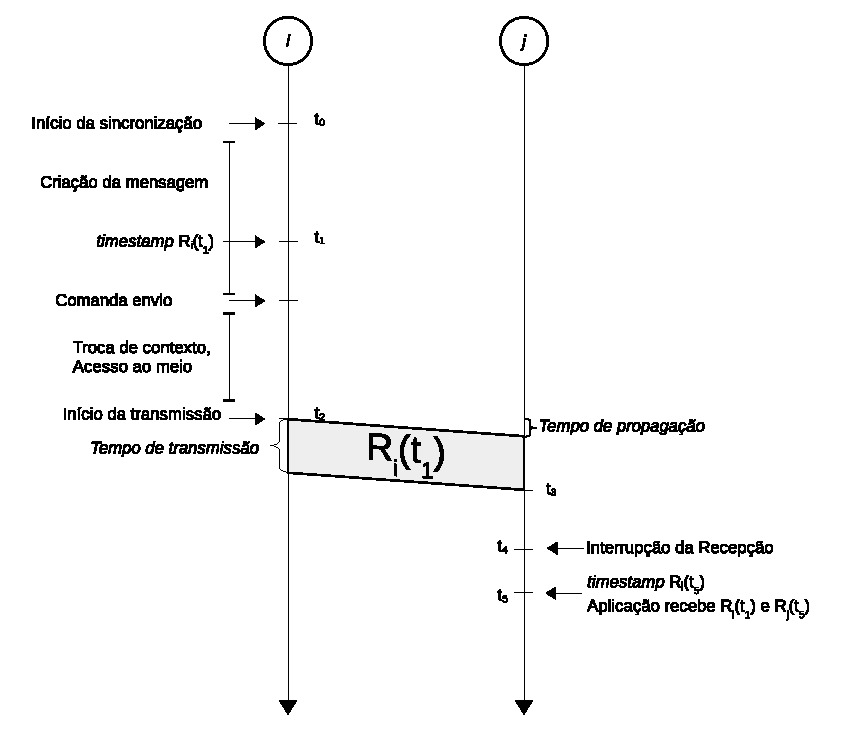
\includegraphics{./figuras/comparacao_mactime.eps}
 % comparacao_mactime.eps: 0x0 pixel, 300dpi, 0.00x0.00 cm, bb=
 \caption{Procedimento de leitura do \textit{timestamp} em n�vel de aplica��o}
 \label{fig:comp_apptimestamp}
\end{figure}




Visando corrigir esse problema, a leitura dos tempos pode ser efetuada em locais mais estrat�gicos. V�rios transmissores tem \textit{chips} capazes de modificar o conte�do da mensagem depois da transmiss�o ter sido iniciada, \textit{timestamps} na camada de acesso ao meio podem ser facilmente implementados nesses dispositivos para eliminar v�rios componentes de atraso.




\begin{figure}[h]
 \centering
 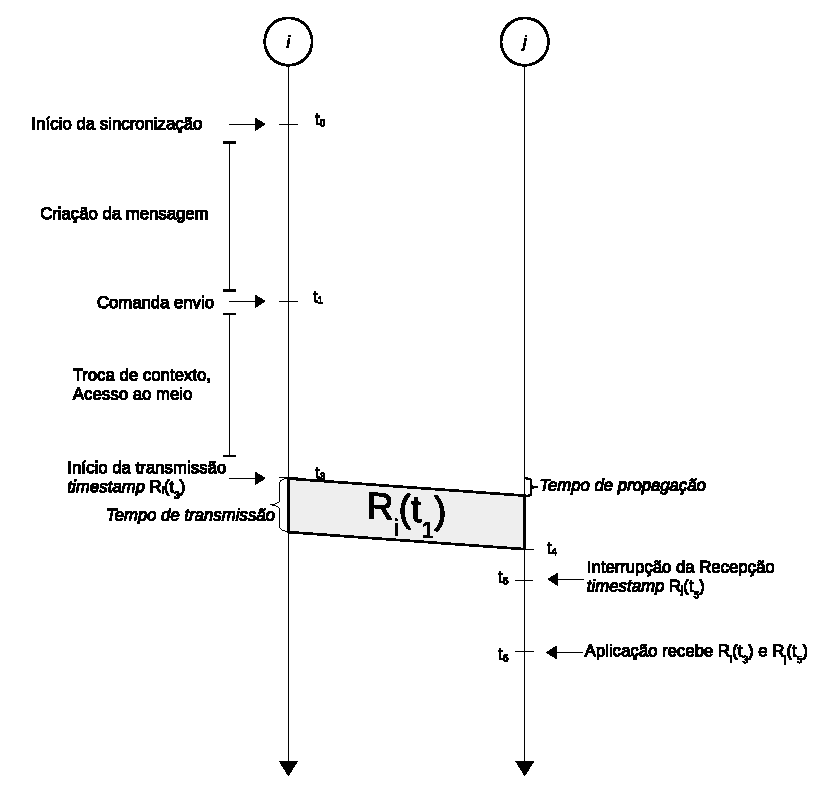
\includegraphics{./figuras/comparacao_mactime2.eps}
 % comparacao_mactime2.eps: 0x0 pixel, 300dpi, 0.00x0.00 cm, bb=
 \caption{Procedimento de leitura do \textit{timestamp} na camada MAC}
 \label{fig:comp_mactimestamp}
\end{figure}




Desta forma, quando � iniciado o processo de transmiss�o a mensagem vai para a fila de sa�da, por�m, quando os primeiros \textit{bits} s�o enviados o \textit{timestamp} � executado. Em um espa�o reservado no \textit{payload} do pacote � inserido uma informa��o adicional de quanto tempo a mensagem levou desde a cria��o at� o envio, procedimento este realizado pelo \textit{chip} de r�dio (uma interrup��o SFD - \textit{Start Frame Delimiter}). Isso permite que o receptor calcule e elimine os atrasos relacionados ao envio. Do lado do receptor � poss�vel usar MAC \textit{timestamp} no momento do recebimento e tamb�m eliminar os atrasos do receptor.

Na Figura \ref{fig:comp_mactimestamp} t�m-se a ilustra��o do procedimento de envio de mensagem de sincroniza��o utilizando \textit{timestamp} na camada MAC. O funcionamento do MAC \textit{timestamp} segue basicamente esse diagrama, onde o n� $i$ inicia o procedimento de envio mensagem de sincroniza��o em $t_0$, logo em seguida cria-se a mensagem e comanda-se o envio. No in�cio da transmiss�o � inserido na mensagem o tempo $t_3$, que � o mesmo instante do in�cio do envio dos dados. J� no lado do receptor, depois do atraso de propaga��o e do tempo de transmiss�o o �ltimo \textit{bit} chega, ent�o uma interrup��o � disparada no tempo $t_5$ junto com ela � registrada o \textit{timestamp} $t_5$.




O formato da mensagem do FTSP segue o modelo da Figura \ref{fig:pacote}. A mensagem come�a com um pre�mbulo, seguido do conjunto de \textit{bytes} de SYNC, um campo de dados e por fim um campo de identifica��o de erros CRC. O PREAMBLE � usado para sincronizar a frequ�ncia dos r�dios, o SYNC � utilizado para calcular o \textit{bit offset} e com isso alinhar os \textit{bytes} no receptor. Os \textit{timestamps} s�o armazenados no limite de cada \textit{byte} transmitido depois de SYNC, tando no envio quanto no recebimento. Os tempos s�o normalizados subtraindo um m�ltiplo inteiro correspondente ao tempo de transmiss�o. Somente o tempo final � inserido no campo de dados da mensagem.

\begin{figure}[H]
 \centering
 \includegraphics{./figuras/ftsp_packet.eps}
 % ftsp_packet.eps: 0x0 pixel, 300dpi, 0.00x0.00 cm, bb=0 0 221 17
 \caption{Formato da mensagem do FTSP}
 \label{fig:pacote}
\end{figure}






A forma como o \textit{timestamp} � realizado depende do modelo do \textit{chip} de r�dio. Pode ser dividido em dois tipos, orientado a \textit{byte} ou orientado pacotes. Nos \textit{chips} orientados a \textit{byte} como o CC1000 \cite{cc1000} (Mica2 e Mica2dot), geram interrup��o por cada \textit{byte} transmitido, essa interrup��o armazena no metadado da mensagem o \textit{timestamp} do momento em que o \textit{byte} foi transmitido ou recebido. Ao final da transmiss�o � poss�vel determinar um \textit{timestamp} �nico, calculando a taxa de transmiss�o e a m�dia dos \textit{timestamps}. Os \textit{chips} CC2420 \cite{chipcon20032} (MicaZ, TelosA, TelosB, TmoteSky) e RF230 (Iris) \cite{iris2006crossbow} s�o orientados a pacote, nesses r�dios ao inv�s de marcarem os tempos em cada \textit{byte} transmitido, fazem apenas uma marca��o para o pacote inteiro usando apenas uma �nica interrup��o SFD.









% Texto da tep 133:
% Several transceivers allow for modifying the contents of a packet after packet transmission is started. Packet-level time synchronization can be implemented very efficiently on such platforms.
% 
% Transmitter's story
% 
% When the communications stack services a TimeSyncAMSend.send command called with event timestamp t\_e, it stores t\_e (e.g. in a map with the pointer of the message\_t as key) and sets the designated timestamp field in the packet payload to 0x80000000.
% When the packet starts being transmitted over the communication medium, a corresponding hardware event is timestamped (e.g. an SFD interrupt). Let us denote this transmission timestamp with t\_tx. The difference of event timestamp t\_e and transmit timestamp t\_tx is written into the designated timestamp field in the payload of the packet (typically into the footer, since the first few bytes might have been transmitted by this time). That is, the information the packet contains at the instance when being sent over the communications medium is the age of the event (i.e. how much time ago the event had occurred).
% If an error occurs with timestamping the transmission or with writing the package payload after transmission has started, then the designated timestamp field in the packet payload will contain 0x80000000, indicating the error to the receiver.
% Receiver's story
% 
% The packet is timestamped with the receiver node's local clock at reception (e.g. with the timestamp of the SFD interrupt). Let us denote the time of reception with t\_rx. The reception timestamp is stored in the metadata structure of the message\_t [5].
% When the event time is queried via the TimeSyncPacket interface, the eventTime command returns the sum of the value stored in the designated timestamp field in packet payload and the reception timestamp, i.e. e\_t- e\_tx+e\_rx. This value corresponds to the time of the event in the receiver's local clock.
% The TimeSyncPacket.isValid command returns FALSE if the time value stored in the payload equals 0x80000000 or if the communications stack failed to timestamp the reception of the packet. Otherwise TRUE is returned, which indicates that the value returned by TimeSyncPacket.eventTime can be trusted.


\section{Escorregamento do Rel�gio}

\outline{
  Descrever os problemas relacionados ao clock drift.
  Como o FTSP corrige essa fonte de imprecis�o.
}

Como apresentado na Se��o \ref{subsec:conceitos}, os sensores de baixo custo apresentam rel�gios muito imprecisos. Cristais de diferentes n�s podem oscilar de forma ligeiramente diferente. Por exemplo, dado um \textit{mote} Mica que tem em sua especifica��o de f�brica a frequ�ncia de $7,3828~MHz$, por�m na verdade ele pode funcionar a $7,3827~MHz$ j� um outro \textit{mote} pode apresentar $7,3829~MHz$, isso gera 20 \textit{ticks} de erro por segundo, este erro acumulado pode atrapalhar a precis�o que se pretende oferecer em uma dada aplica��o. Esse comportamento causa a necessidade de ressincroniza��o em per�odos mais curtos. 

\begin{figure}[h]
 \centering
 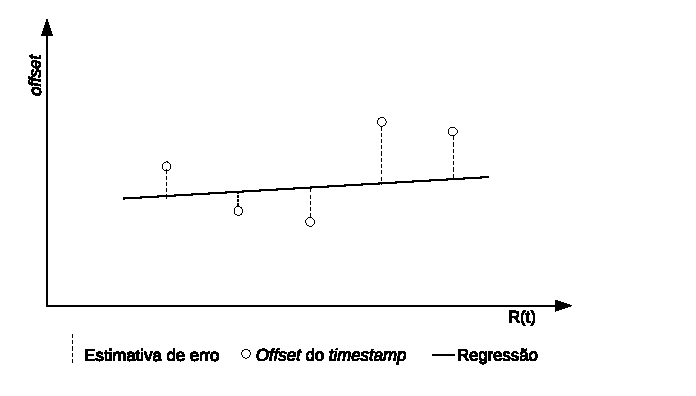
\includegraphics{./figuras/grafico_regressao.eps}
 % grafico_regressao.eps: 0x0 pixel, 300dpi, 0.00x0.00 cm, bb=
 \caption{Regress�o linear aplicada a \textit{timestamps}}
 \label{fig:regressao}
\end{figure} 

Regress�o linear � o m�todo mais utilizado para estimar o desvio do rel�gio de um n� para com o rel�gio da raiz \cite{maroti2004}. No processo de sincroniza��o um n� de refer�ncia ou \textit{root}, envia seu uma mensagem com seu pr�prio tempo, os receptores usam esse tempo para iniciar seu rel�gio local. Ent�o o \textit{root} passa a enviar periodicamente seu \textit{timestamp}, cada um dos receptores armazenam em uma tabela os tempos recebidos junto com o tempo de recebimento baseado no seu rel�gio local. A predi��o de erro � a diferen�a entre o tempo de refer�ncia do n� \textit{root} e a estimativa de tempo do n� receptor.

De acordo com \cite{capriglione2016}, usando regress�o linear � poss�vel predizer um padr�o pelo calculo dos pares de \textit{timestamps} recebidos, e utiliz�-los para compensar os erros. Uma linha de regress�o linear fornece a inclina��o necess�ria para estimar o tempo do n� \textit{root} no futuro, a Figura \ref{fig:regressao} ilustra esse processo. Assim, � poss�vel ajustar de forma mais suave a taxa de crescimento do rel�gio para algo mais pr�ximo na no��o global de tempo. No FTSP devido as limita��es de mem�ria dos dispositivos o tamanho padr�o das tabelas � 8 pares de \textit{timestamps}, os autores comprovaram em experimentos que a taxa de erro utilizando essa t�cnica � de $1.48\mu s$ em m�dia, quando desligado o recurso o erro passa a ser crescente e acumula com o tempo.






\section{Sincroniza��o Multi-saltos}

\outline{
\begin{itemize}
 \item Formato da mensagem de sincroniza��o.
 \item Gerenciamento de informa��o redundante.
 \item Elei��o do n� raiz.
 \item Evento: enviar/receber mensagem de sincronia. 
\end{itemize}

}



% \begin{figure}[h]
%  \begin{Verbatim}[numbersep=1pt,frame=single]
% typedef nx_struct TimeSyncMsg
% {
%  nx_uint16_t rootID;
%  nx_uint16_t nodeID; 
%  nx_uint8_t  seqNum;
%  nx_uint32_t globalTime;
%  nx_uint32_t localTime;
% } TimeSyncMsg;
% \end{Verbatim}
% \caption{Formato da mensagem de sincroniza��o}
% \end{figure}




%This section briefly describes the Flooding Time Synchronization Protocol (FTSP). For more detailed information, refer to \cite{maroti2004}.

% FTSP is a synchronization protocol for WSN that provides high accuracy, consumes few resources, uses little bandwidth and is fault-tolerant. It elects a node as root to provide the time reference for synchronization; if root failure is detected (using timeouts), another root is elected.
% Root and synchronized nodes send synchronization messages periodically, and receiving nodes use these messages to synchronize.
% Therefore, FTSP supports multi-hop networks.
% 
% Synchronization messages comprise a \textit{sender timestamp} which is the estimated global time and \textit{rootID} which is the network identifier of the root (where the node with the lowest ID is the chosen root).
% \textit{seqNum} is a sequence counter that is incremented each synchronization round; this field is used to verify the redundancy of messages \cite{maroti2004}.
% 
% All nodes think they are root when the network starts, so they broadcast synchronization messages to the network. 
% When they receive a synchronization message, they check who has the lowest ID: if the local ID is higher, this node gives up on being root and starts synchronizing.
% Another important check is the \textit{seqNum}.
% If it is greater than the local value \textit{highestSeqNum}, it means that this is a new synchronization message and starts the synchronization procedure.
% 
% The synchronization procedure consists of computing a linear regression \cite{elson2003} that will provide the clock skew (used to estimate the global time) in relation to the reference node.
% The last step is to forward its local (synchronized) time to other nodes. 


%%A mensagem de sincroniza��o compreende um \textit{timestamp} do emissor, que � estimativa de tempo global e \texttt{rootID} que � 


% \begin{figure}[h]
%  \centering
%  \includegraphics{./figuras/exemplo_ftps1.eps}
%  % exemplo_ftps1.eps: 0x0 pixel, 300dpi, 0.00x0.00 cm, bb=0 0 330 180
%  \caption{Exemplo do fluxo da rede com FTSP}
%  \label{fig:exemplo_ftsp1}
% \end{figure}


\begin{figure}[h]
\begin{Verbatim}[numbers=left,numbersep=1pt,frame=single]
event Radio.receive(TimeSyncMsg *msg){
  if( msg->rootID < myRootID )
      myRootID = msg->rootID;
  else if( msg->rootID > myRootID
    || msg->seqNum <= highestSeqNum )
      return;
  highestSeqNum = msg->seqNum;
  if( myRootID < myID )
      heartBeats = 0;
  if( numEntries >= NUMENTRIES_LIMIT
    && getError(msg) > TIME_ERROR_LIMIT )
      clearRegressionTable();
  else
      addEntryAndEstimateDrift(msg);
}
\end{Verbatim} 
 \caption{FTSP Receive Routine \cite{maroti2004} }%\vspace{0em}
 \label{figure1}
\end{figure}


A Figura \ref{figure1} mostra a rotina de recebimento de mensagens de sincroniza��o. 
As linhas 2 e 3 comparam o \texttt{rootID} da mensagem de sincroniza��o recebida com a informa��o local que o n� tem sobre que � o \textit{root} \texttt{myRootID}.
Se a mensagem recebida tem o \texttt{rootID} menor, o n� assume \texttt{rootID} como seu root.
As linhas de 4 a 7 ignoram as mensagens que tenham um \texttt{rootID} e \texttt{seqNum} menores, pois possuem informa��o irrelevante.
Se \texttt{seqNum} � maior, o valor de \texttt{highestSeqNum} � atualizado.
Linhas 8 e 9 fazem o n� \textit{root} desistir de ser a \textit{root} da rede quando existe um \texttt{rootID} menor que seu pr�prio ID.
No caso de \texttt{rootID} ser maior que o verificado se o \texttt{seqNum} � maior ou igual ao valor do \texttt{highestSeqNum}, esta checagem previne informa��es redundantes por que a mensagem ser� apenas usada quando o \texttt{rootID} for menor ou igual a \texttt{myRootID} e o numero maior que o valor de \texttt{highestSeqNum}.
Linhas 10 e 15 verificam se o tempo da mensagem est� em discord�ncia com a estimativa de tempo global mais recente, se � aplic�vel limpa a tabela de regress�o, se n�o, acumula a mensagem para calcular a regress�o linear e sincronizar.
As linhas 10 a 15 armazenam mensagens de sincroniza��o para calcular a regress�o linear e realizar a sincroniza��o.

% Figure \ref{figure1} shows the routine of receiving synchronization messages.
% Lines 2 and 3 compare the \textit{rootID} of the synchronization message with the local \textit{rootID}.
% If the message has a lower \textit{rootID}, the node assumes this \textit{rootID} as root.
% Lines 4 to 7 ignore messages with higher  \textit{rootID} and lower \textit{seqNum}.
% If \textit{seqNum} is higher, local \textit{highestSeqNum} is updated.
% Lines 8 and 9 makes a root node give up on being root when it has a \textit{rootID} lower than its own ID.
% In case the \textit{rootID} is larger it is checked whether the \textit{seqNum} is greater or equal to the value of \textit{highestSeqNum}, this check prevents information redundancy because the message will only be used when the \textit{rootID} is less than or equal to \textit{myRootID} and the number greater than the value of \textit{highestSeqNum}.
% Lines 10 to 15 verify if the time of a message is in disagreement with the earlier estimates of global time, if applicable clear the regression table, if not, accumulate synchronization messages to calculate the linear regression and synchronize.
%Lines 10 to 15 accumulate synchronization messages to calculate the linear regression and synchronize.



\begin{figure}[h]
   \begin{Verbatim}[numbers=left,numbersep=1pt,frame=single]
event Timer.fired() {
  ++heartBeats;
  if( myRootID != myID
    && heartBeats >= ROOT_TIMEOUT )
      myRootID = myID;
  if( numEntries >= NUMENTRIES_LIMIT
    || myRootID == myID ){
      msg.rootID = myRootID;
      msg.seqNum = highestSeqNum;
      Radio.send(msg);
  if( myRootID == myID )
      ++highestSeqNum;
  }
}
  \end{Verbatim}
  \caption{FTSP Send Routine \cite{maroti2004}}
  \label{figure2}
\end{figure}

A Figura \ref{figure2} mostra a rotina de envio de mensagem. 
Um n� decide tornar-se \textit{root} por que est� sem receber mensagens de sincroniza��o por \texttt{ROOT\_TIMEOUT} (linhas 3 a 5).
Um n� envia mensagens de sincroniza��o se ele � o \textit{root} ou se est� sincronizado (linhas 6 a 10).
Se um n� � o \textit{root}, ele tamb�m tem que incrementar seu \textit{highestSeqNum}.
% Figure \ref{figure2} shows the sending routine.
% A node decides to be root because has not received a synchronization message for ROOT\_TIMEOUT (lines 3 to 5).
% A node sends synchronization messages if it is root or has synchronized (lines 6 to 10).
% If a node is root, it also has to increment its \textit{highestSeqNum}. 


 
 


\chapter{FTSP+} \label{cap:cap4}
\outlineon=1

\outline{Intro}

\outline{
  \begin{itemize}
    \item Explicar a t�cnica.
    \item Inserir ilustra��o do processo de sincroniza��o com o rel�gio externo. 
    \item Pseudo c�digo
    \item FTSP+ e subsection
  \end{itemize}
}

\section{T�cnica}

\outline{Descrever o processo de c�lculo do tempo de acesso ao meio, e onde foi baseado.}


\section{Modifica��o}

\outline{
   Pseudo c�digo com explica��o do passo-a-passo do algoritmo (no sender e no receiver).
}


\chapter{Implementa��o}
\outlineon=0


\outline{
  Descrever o processo de Implementa��o no tinyos (libs, organiza��o do c�digo e TEPs).
  
}

Este cap�tulo trata sobre o sistema operacional TinyOS a linguagem nesC e os dispositivos de \textit{hardware}. Aspectos importantes de sua arquitetura para a implementa��o de um protocolo de sincroniza��o. 



\section{Mote}\label{sec:mote}

O termo \textit{mote} � utilizado para se referir ao dispositivo que � n� em uma rede de sensores sem fio, foi introduzido por pesquisadores da Universidade de Berkeley \cite{culler2002mica} no in�cio da d�cada de 90, assim, constantemente podemos encontrar refer�ncias como ``Berkeley Mote'' para designar estes dispositivos de rede, independente do fabricante. 

O MicaZ � um \textit{mote} dispon�vel comercialmente e amplamente utilizado em pesquisas acad�micas. Possui um processador de 4 MHz com 8 \textit{bits}, mem�ria de 128 kB. A diferen�a comparado a um computador com a capacidade similar do in�cio da d�cada de 1980, como o 8088, � o baixo consumo de energia que varia de 15 $\mu$A no modo de economia at� 8 mA em execu��o. Outro componente significativo � o r�dio, esses dispositivos possuem transmissores com frequ�ncia de 2.4 GHz e taxa de dados de 250 kbps, usam a estrat�gia de acesso ao meio CSMA/CA, conseguindo transfer�ncias de 40.000 bps.


\begin{table}[h]
\centering
\begin{tabular}{lcc}
\hline
\textbf{Item}         & \textbf{MicaZ}              & \textbf{Iris}\\
\hline
Processador           & ATMega 128L 8MHz            & ATmega1281 16MHz                                                                  \\
\textit{Flash}        & \multicolumn{2}{c}{128 kB}                                                                                                                                                           \\
Mem�ria Dados         & \multicolumn{2}{c}{512 kB}                                                                                                                                                           \\
EEPROM                & \multicolumn{2}{c}{4 kB}                                                                                                                                                             \\
ADC                   & \multicolumn{2}{c}{10 bit}                                                                                                                                                           \\
\textit{Chip} de R�dio         & CC2420                     & RF230                                                                             \\
Frequ�ncia do R�dio   & \multicolumn{2}{c}{2.4 GHz}                                                                                                                                                          \\
Taxa de Transfer�ncia & \multicolumn{2}{c}{250 kbps}                                                                                                                                                         \\
Voltagem de Opera��o  & \multicolumn{2}{c}{3,6 - 2,7}                                                                                                                                                        \\
Consumo de Energia    & \begin{tabular}[c]{@{}c@{}}RX 19,7 mA\\ TX 17,4 mA\\ \textless 15 $\mu$A (dormindo)\end{tabular} & \begin{tabular}[c]{@{}c@{}}RX 16 mA\\ TX 17 mA\\ 8 $\mu$A (dormindo)\end{tabular}\\
\hline
\end{tabular}
\caption{Especifica��es de \textit{hardware} dos \textit{motes}}
\label{tab:micazxiris}
\end{table}

A jun��o destas caracter�sticas, fornecem recursos que tornam o \textit{mote} uma boa op��o para diversas aplica��es, a capacidade de computa��o o consumo de energia trazem a flexibilidade para implanta��o destes equipamentos em RSSF, a Tabela \ref{tab:micazxiris} cont�m as especifica��es dos \textit{hardwares} utilizados.





\section{Sistema Operacional}

\outline{
\begin{itemize}
 \item Gerencia de mem�ria. Gerenciamento energ�tico. Redes. Linguagem. Manipula��o de interrup��es. Programa��o baseada em eventos.
\end{itemize}    
}


%\cite{levis2004tinyos}
%\cite{gay2003nesc}
%We present nesC, a programming language for networked embedded systems that represent a new design space for application developers. An example of a networked embedded system is a sensor network, which consists of (potentially) thousands of tiny, low-power "motes," each of which execute concurrent, reactive programs that must operate with severe memory and power constraints.nesC's contribution is to support the special needs of this domain by exposing a programming model that incorporates event-driven execution, a flexible concurrency model, and component-oriented application design. Restrictions on the programming model allow the nesC compiler to perform whole-program analyses, including data-race detection (which improves reliability) and aggressive function inlining (which reduces resource consumption).nesC has been used to implement TinyOS, a small operating system for sensor networks, as well as several significant sensor applications. nesC and TinyOS have been adopted by a large number of sensor network research groups, and our experience and evaluation of the language shows that it is effective at supporting the complex, concurrent programming style demanded by this new class of deeply networked systems.


O desenvolvimento do FTSP+ foi realizado utilizando o sistema operacional TinyOS, que � um SO bem difundido na �rea de redes sensores sem fio \cite{levis2004tinyos}. O TinyOS n�o � um sistema operacional convencional, em que se instala completamente no sensor, ele se apresenta como um arcabou�o de um conjunto de componentes reutiliz�veis que permitem o desenvolvimento de aplica��es para sistemas embarcados em conjunto com o SO. Esses componentes s�o separados por fun��es caracter�sticas, no momento de construir a aplica��o somente os componentes especificados ser�o integrados na aplica��o final, mantendo o uso minimal de recursos. 

Com a limita��o de recursos nos dispositivos sensores o TinyOS conta com pouco menos de 400 \textit{bytes} de tamanho, � um sistema baseado em eventos, com suporte a concorr�ncia, eventos ass�ncronos e comandos. Um programa em TinyOS possui a abstra��o dos componentes em um modelo de grafo, como vemos na Figura \ref{fig:diagrama_componentes}.


As aplica��es e o pr�prio sistema operacional s�o escritos em nesC (\textit{networked systems C}) \cite{gay2003nesc} um dialeto da linguagem C, que d� o suporte a arquitetura de componentes e orienta��o a eventos, al�m de ser otimizada para reduzir o consumo de mem�ria e ter primitivas que previnam problemas de baixo n�vel como condi��o de corrida. No desenvolvimento existe a separa��o da organiza��o dos componentes e programa��o das interfaces, os componentes s�o conectados (\textit{wired}) juntos em um arquivo de aplica��o, j� o c�digo dos eventos e tarefas s�o feitos em um arquivo de constru��o.


%Como o TinyOS tem o c�digo aberto, � poss�vel alter�-lo e criar ou estender suas funcionalidades.

Programas em nesC s�o constru�dos por itens definidos separadamente e ent�o conectados de forma explicita para juntar todos em uma unidade \cite{levis2009tinyos}. A seguir defini��es importantes sobre essas caracter�sticas:

\begin{itemize}
 \item Componentes e interfaces: Um programa em nesC � um conjunto de componentes ligados entre si. O componente fornece interfaces que s�o respons�veis pela comunica��o bidirecional entre os componentes, as interfaces fornecem comando e eventos.
 
 \item Implementa��o: A implementa��o pode ser dividida em duas partes no nesC, uma chamada \textit{modules} e outra \textit{configuration}. Em \textit{modules} � implementado as interfaces, j� em \textit{configuration} � usado para juntar os componentes conectando suas interfaces.
 
 \item Modelo de concorr�ncia: Define como os componentes interagem entre suas execu��es. Temos dois tipos de tarefa, que s�o a tarefa (ou \textit{task}) propriamente dita e eventos de dispositivos. Quando uma tarefa � enviada para execu��o ela roda at� completar, n�o fazendo preemp��o. Os eventos de dispositivos s�o como as tarefas, s� que s�o geradas como respostas a eventos.
\end{itemize}







\section{Diagramas e Componentes}\label{sec:dia}

\outline{
  O Tinyos tem o recurso de componentes para disponibilizar seus mais diversos recursos, descrever os componentes relevantes para o trabalho e os componentes resultantes das altera��es.
}

O TinyOS foi desenvolvido seguindo um conjunto de diretrizes, chamado de TEP (TinyOS Enhancement Proposals) que orientam as modifica��es no n�cleo do seu c�digo, tamb�m � utilizado para guiar a cria��o de novas funcionalidades. Podemos citar as seguintes TEPs \cite{tinyos133, tinyos132, tinyos102} com defini��es importantes para a implementa��o do FTSP+:

\begin{itemize}
 \item TEP 102: Prop�e a estrutura dos \texttt{Timers} (controladores do rel�gio) e suas propriedades de precis�o, acur�cia e tamanhos.
 \item TEP 132: Descreve o mecanismo de \textit{timestamp} no n�vel de acesso ao meio. A funcionalidade que fornece o tempo de envio e recebimento de uma mensagem no processo de comunica��o.
 \item TEP 133: Descreve o funcionamento do mecanismo das mensagens de sincroniza��o de tempo, como os tempos s�o convertidos do tempo do emissor para o do receptor e como s�o tratados nas pilhas de protocolos.
\end{itemize}

Os \textit{Timers} no TinyOS fornecem precis�es listadas na Tabela \ref{tab:precision}, todas as precis�es s�o bin�rias, ou seja, 1s cont�m 1024 milissegundos bin�rios. A acur�cia dependente de qu�o bem o dispositivo fornece de seu rel�gio, como vimos anteriormente os rel�gios s�o afetados pelas limita��es de seu \textit{hardware}. Assim um rel�gio de um \textit{mote} que roda a 7.37MHz, tem valor real do rel�gio variando muito pr�ximo desse valor. Os tamanhos s�o basicamente 8, 16, 32 e 64 \textit{bits}, sendo 32 \textit{bits} o tamanho indicado para representa��o dos tempos dos componentes.

\begin{table}[h]
\centering
\begin{tabular}{lccc}
Nome & TMilliC & T32kHz & TMicroC \\
\hline
Frequ�ncia & 1,024 Hz & 32,768 Hz & 0.9216 MHz \\
\hline
Precis�o & 1024 ticks/s & 32768 ticks/s & 1048576 ticks/s \\
\hline
Periodo & 976 ms & 30.518 $\mu s$ & 1.084 $\mu s$
\end{tabular}
\caption{Precis�es dos \textit{Timers} no TinyOS}
\label{tab:precision}
\end{table}%alemao


O FTSP+ foi elaborado utilizando os \textit{motes} Iris e Micaz \cite{Iris2007, Micaz}, e constru�do sobre a implementa��o j� existente do FTSP. A Figura \ref{fig:diagrama_componentes} apresenta os componentes utilizados pelo FTSP+, a altera��o descrita na Se��o \ref{sec:mod} est�o presentes no componente central da imagem o \texttt{TimeSyncP}.



\begin{figure}[h]
 \centering
 %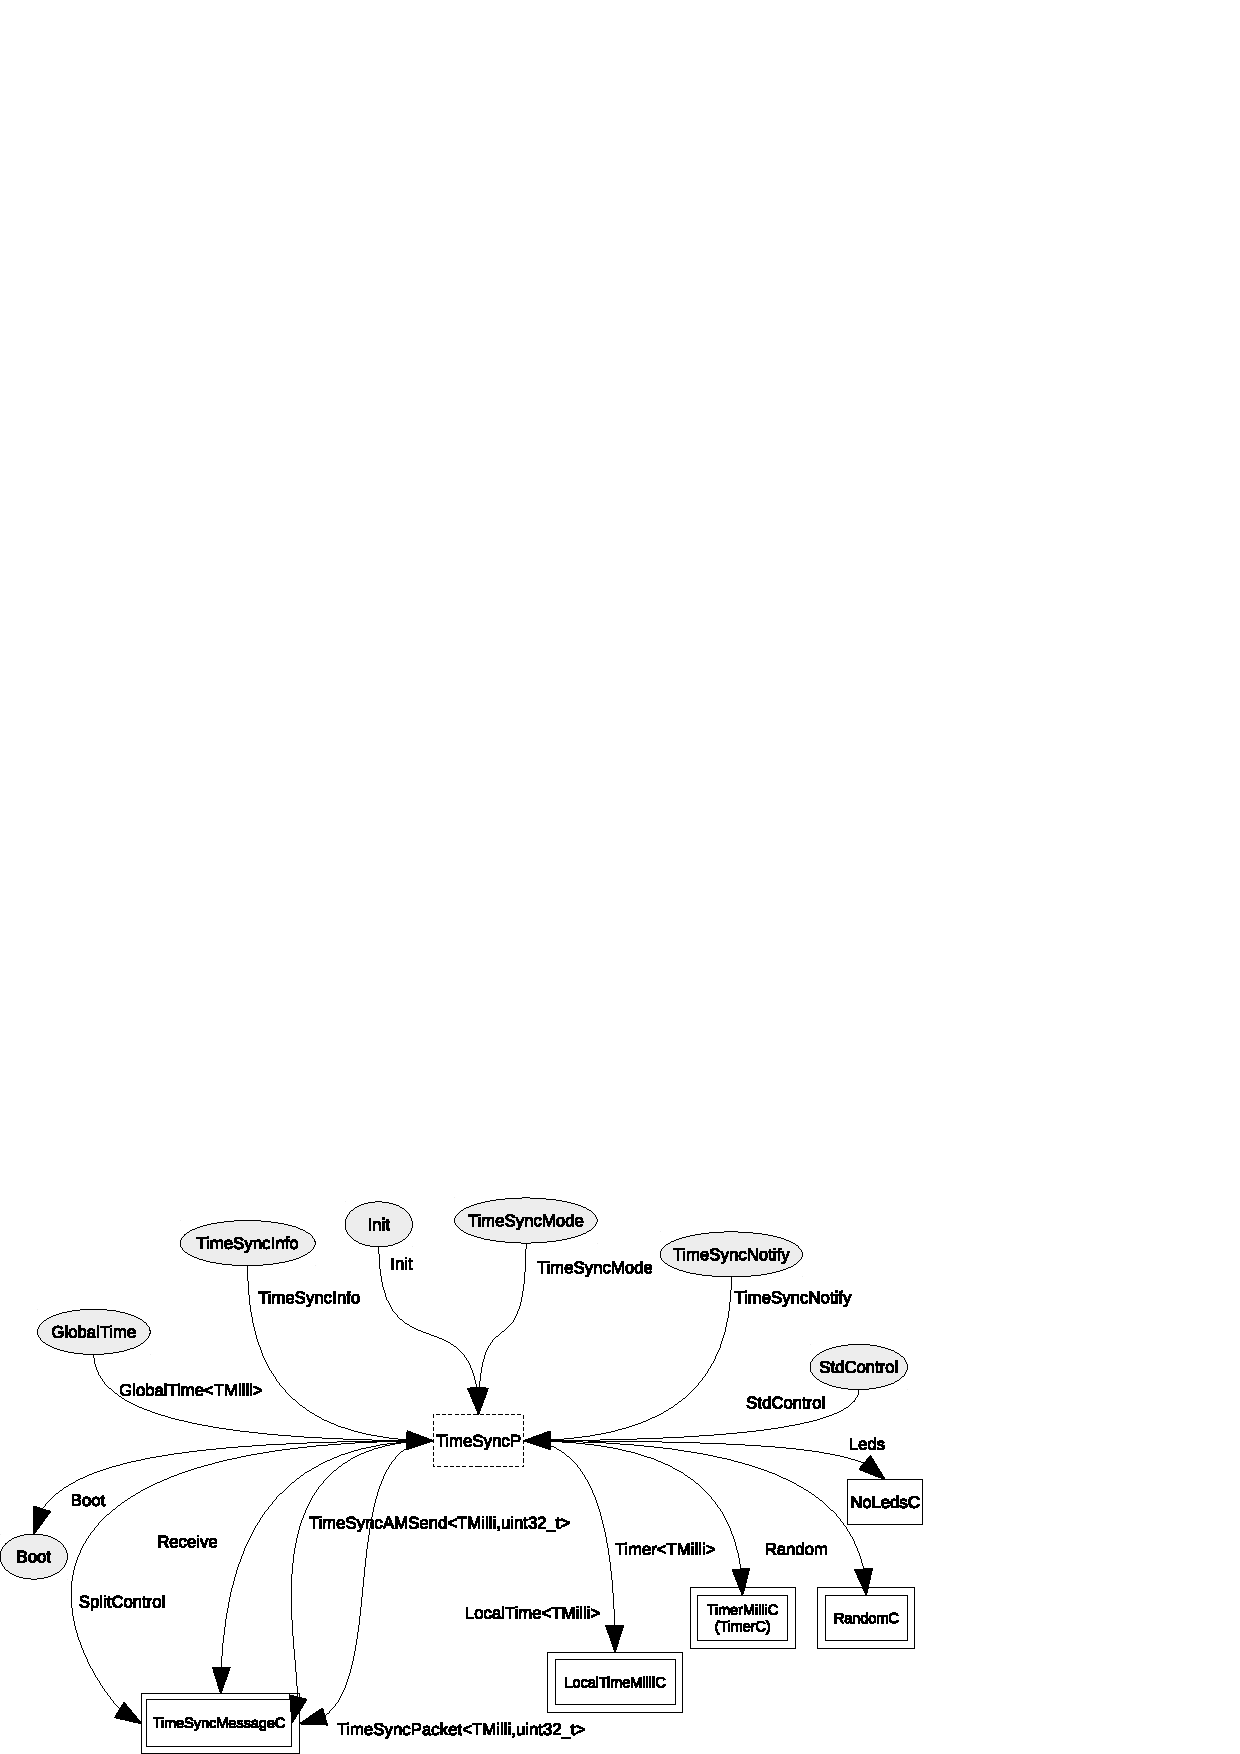
\includegraphics[width=23cm, angle=90]{./figuras/time.png}
 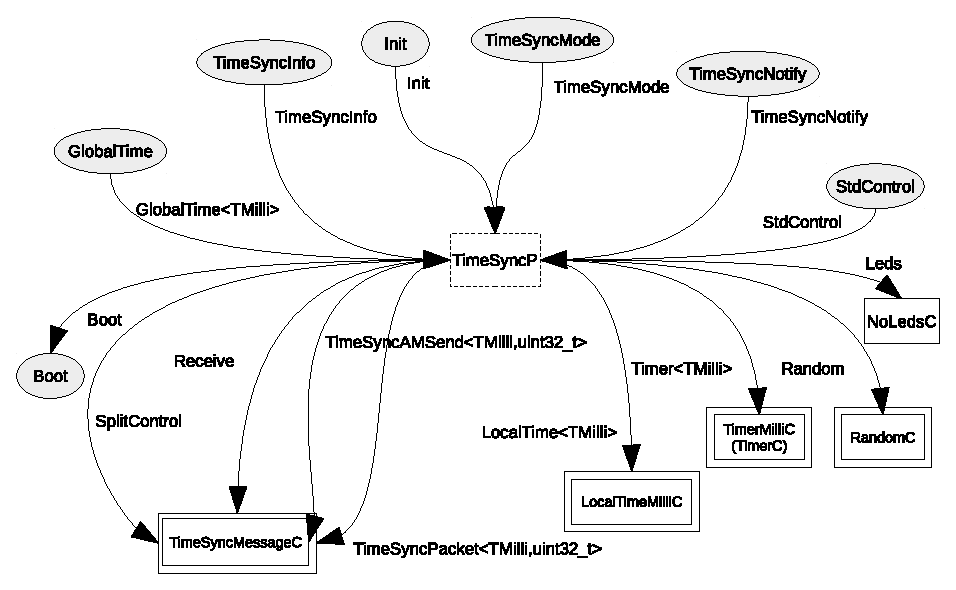
\includegraphics{./figuras/time.eps}
 % tos.lib.ftsp.TimeSyncC.png: 1177x293 pixel, 72dpi, 41.52x10.34 cm, bb=0 0 1177 293
 \caption{Diagrama de Componentes do FTSP+}
 \label{fig:diagrama_componentes}
\end{figure}

O \texttt{TimeSyncP} faz parte a implementa��o original do FTSP, por�m foi o �nico componente modificado. O FTSP usa uma mensagem de sincroniza��o com informa��es como o n� raiz da rede, o n� que est� enviando a mensagem de sincroniza��o, o n�mero de sequ�ncia da mensagem e o \textit{timestamp}. � acrescentado mais uma mensagem na comunica��o, que � a mensagem de corre��o. A estrutura da mensagem � listada a seguir:

% \begin{figure}[h]
%  \begin{Verbatim}[numbersep=1pt,frame=single]
% typedef nx_struct TimeSyncMsg
% {
%  nx_uint16_t rootID;
%  nx_uint16_t nodeID; 
%  nx_uint8_t  seqNum;
%  nx_uint32_t globalTime;
%  nx_uint32_t localTime;
% } TimeSyncMsg;
% \end{Verbatim}
% \caption{Formato da mensagem de sincroniza��o}
% \end{figure}

\begin{figure}[h]
 \begin{Verbatim}[numbersep=1pt,frame=single]
typedef nx_struct TimeSyncMsg
{
 nx_uint16_t rootID;
 nx_uint16_t nodeID;      
 nx_uint8_t  seqNum;
 nx_uint32_t correction; 
} TimeSyncMsg;
\end{Verbatim}
\caption{Formato da mensagem de sincroniza��o}
\end{figure}


O mensagem conta com o \texttt{rootID}, se a mensagem tem \textit{root} com ID maior que a informa��o do \textit{root} local ela � descartada. O \texttt{nodeID} cont�m o ID de quem enviou a mensagem. O \texttt{seqNum} serve para identificar qual o \textit{timestamp} a mensagem est� corrigindo. O campo \texttt{correction} � o campo que traz a estimativa de erro do emissor e � com ele que ser� feita a corre��o dos \textit{timestamp} anteriormente recebidos.

No documento da TEP 132 \cite{tinyos132}, � fornecido uma breve descri��o sobre o padr�o de \textit{timestamps} oferecidos pela interface \texttt{PacketTimeStamp} que faz o acesso ao tempo de recep��o e envio de determinada mensagem.

A TEP 133 fornece a abstra��o para o mecanismo de sincroniza��o de pares. N�o prov� um sincroniza��o completa da redes, mas, com seus recursos � poss�vel implementar um servi�o de sincroniza��o completo, exemplo o FTSP, pois os componentes e interfaces utilizados em sua implementa��o est�o bem definidos em seu documento \cite{tinyos133}. 

Outro aspecto importante da TEP 133 � o seu guia de implementa��o, que compreende duas abordagens, uma em que � poss�vel mudar o \textit{payload} da mensagem durante a transmiss�o usando a interrup��o SFD dos r�dios orientados a pacote. A segunda abordagem descreve a possibilidade da sincroniza��o para plataformas em que n�o seja poss�vel a altera��o do conte�do durante a transmiss�o. Podemos verificar que o FTSP atende a primeira abordagem, j� a segunda n�o � atendida, por�m com o FTSP+ ambas as abordagens s�o acolhidas.


O pr�ximo cap�tulo traz experimento realizado com \textit{motes} reais, e gr�ficos estat�sticos dos resultados encontrados. Os experimentos foram baseados nas t�cnicas desenvolvidas at� aqui.

\chapter{Experimentos} \label{cap:cap5}
\outlineon=0

\outline{
Listar o experimentos de maneira num�rica 1,2 e 3. Em cada item explicar os exp em si.
\begin{itemize}
 \item O que eu quero responder com os experimentos.
 \item Quais m�tricas utilizar.
 \item Definir ambiente.
 \item Colocar os gr�ficos e tabelas gerados pelos experimentos.
 \item Comentar e analizar os resultados.
\end{itemize}

}

Neste cap�tulo nos descrevemos nossos experimentos a respeito da precis�o do FTSP+. N�s implementamos o FTSP+ sobre TinyOS 2.1.2 \cite{levis2004tinyos} e executamos os testes em \textit{motes} Micaz \cite{Micaz}.
% In this section, we describe our experiments to assess FTSP+'s accuracy.
% We have implemented FTSP+ on TinyOS 2.1.2 \cite{levis2005tinyos} and ran our tests on Micaz motes \cite{micaz}.


%\section{Experimento 1}\label{exp:1}

\outline{
    Descrever o ambiente, tipo de sensor, tempo de dura��o e demais caracteristicas do cen�rio testado.
}

Os \textit{motes} Micaz suportam o \textit{timestamp} na camada MAC, mas n�s precisamos desta informa��o para medir a acur�cia da nossas precis�o.
Para a sincroniza��o, n� reescrevemos o recurso de MAC \textit{timestamp} com o nosso \textit{timestamp} na camada de aplica��o.
% Micaz motes do support MAC layer timestamping, but we need this information to measure our correction accuracy.
% For synchronization, we overwrite MAC timestamp with our application layer timestamp.


N�s usamos \textit{jiffys} como unidade de tempo por que esta � base de tempo do TinyOS e representa o tempo entre 2 \textit{ticks} do rel�gio.
Nossos experimentos s�o resultados de uma rede com os n�s trocando mensagens de sincroniza��o a cada 3 segundos durante 10 minutos.
% We use \textit{jiffys} as time unit because this is the time basis of TinyOS and represents the time between 2 clock ticks.
% Our experiments results correspond to 10 minutes experiments with synchronization messages being sent every 3 seconds.


\begin{figure}[htb!]
	\centering
		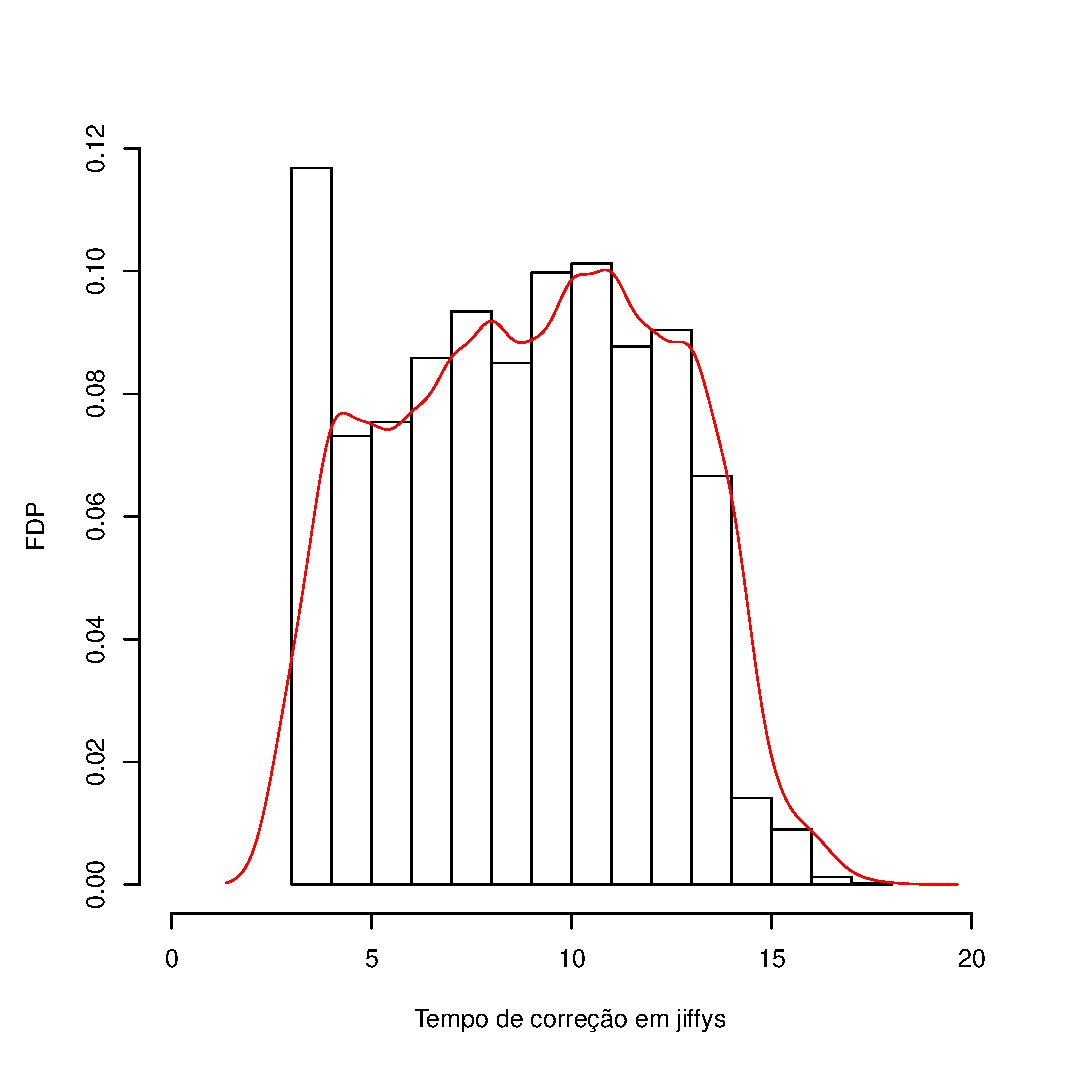
\includegraphics[width=\linewidth]{./figuras/correction_distribution.eps}
	%\caption{Histogram and P.D.F. of correction times.}
	\caption{Histograma e F.D.P. dos tempos de corre��o.}
	\label{fig:correction_hist}
\end{figure}

\begin{figure}[htb!]
	\centering
		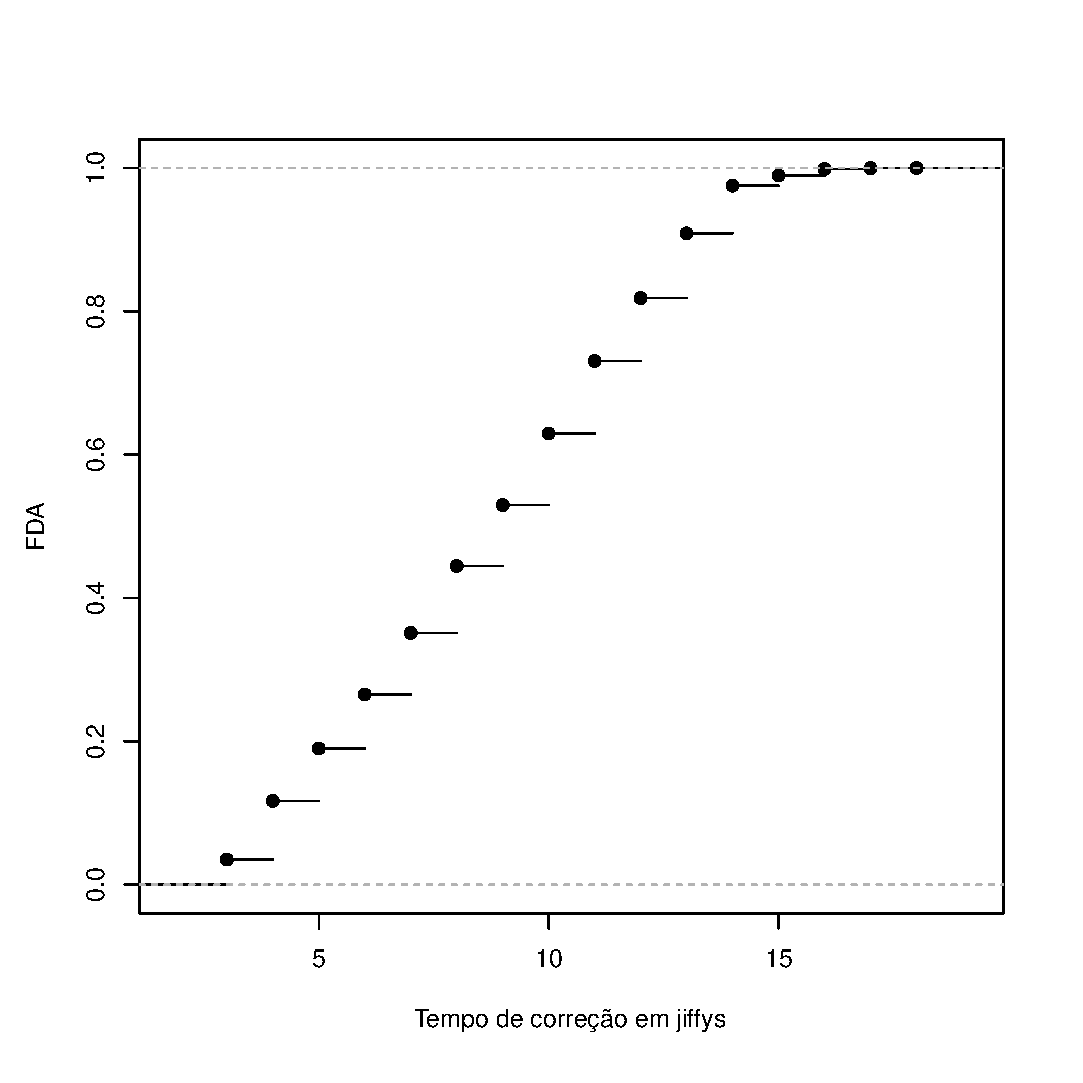
\includegraphics[width=\linewidth]{./figuras/correction_cdf.eps}
	%\caption{C.D.F. of correction times.}
	\caption{F.D.A. dos tempos de corre��o.}
	\label{fig:correction_cdf}
\end{figure}


 \begin{table}[htb!]
 \centering
 \begin{tabular}{c|c|c}
 		& \multirow{2}{*}{\textbf{M�dia ($\mu{s}$)}}	& \multirow{2}{*}{\textbf{Desvio padr�o}} \\
		&&\\
 $\mathbf{tempo~de~processamento}$ 	&  $0.87 \pm 0.0095$ 	& $0.33$\\
 $\mathbf{\delta}$  	&  $0.88 \pm 0.0093$ 	& $0.33$\\
 $\mathbf{tempo~de~corre��o}$ 	& $9.01 \pm 0.093$	& $3.32$\\
 $\mathbf{acesso~ao~meio}$ 	& $8.13 \pm 0.093$	& $3.31$\\
 $\mathbf{t4' - \bar{t4'}}$ 	& $-0.0047 \pm 0.013$ 	& $0.47$ \\
 \end{tabular}
 %\caption{Mean and standard deviation}
 \caption{M�dia e desvio padr�o.}
 \label{tab:mean_sd}
 \end{table}

Nosso primeiro mediu a distribui��o de probabilidade dos tempos de corre��o (relembrando da Se��o \ref{sec:mod} que � $t_2-t_1+\delta$).
Como podemos ver na Figura \ref{fig:correction_hist}, os tempos de corre��o variam na maioria de 5 at� 13 \textit{jiffys} com uma distribui��o uniforme.
N�s podemos ver na Figura \ref{fig:correction_cdf}, que mostra a fun��o distribui��o acumulada da corre��o dos tempos, que est� em cerca de 80\% dos casos de corre��o de tempo acima de 5 \textit{jiffys}.
Isto � um \textit{overhead} significante e uma fonde de imprecis�o que o FTSP+ � capaz de medir e fazer uma compensa��o.
Para nosso cen�rio a m�dia de corre��o de tempo de atraso � $9.01$\footnote{Este valor � dependente de cen�rio enquanto depende da janela de conten��o da rede.} \textit{jiffys} como vemos na Tabela \ref{tab:mean_sd} onde podemos ver que temos a m�dia com intervalo de confian�a de $95\%$ e desvio padr�o.

% Our first experiment measures the probability distribution of correction times (recall from Section \ref{sec:mod} that it is $t2-t1+\delta$).
% As can be seen in Figure \ref{fig:correction_hist}, correction time varies mostly from 5 to 13 jiffys with an uniform distribution.
% We can see in Figure \ref{fig:correction_cdf}, which plots the cumulative density function of the correction times, that in about 80\% of cases correction time is above 5 jiffys.
% This is a significant overhead and source of inaccuracy that FTSP+ is able to measure and compensate for. 
% For our scenario the average correction time delay is $9.01$\footnote{This value is scenario-dependent while it depends upon the scenario contention level.} jiffys as we can see in Table \ref{tab:mean_sd} where we have the mean with confidence interval of $95\%$ and the standard deviation.



\begin{table}[htb!]
\centering
\begin{tabular}{l|c|c|c|c|c|c}
\textbf{Atraso em jiffys} 			& 0 		& 1 			& 2 & 3 & 4 & 5 \\
\textbf{Frequ�ncia} 	& 606 	& 4271  & 0 & 1 & 1 & 1 \\
\end{tabular}
%\caption{Delay frequency of receiver \textit{processing time}.}
\caption{Frequ�ncia de atraso do receptor \textit{tempo de processamento}.}
\label{tab:processing_time}
\end{table}

\begin{table}[htb!]
\centering
\begin{tabular}{l|c|c|c|c|c|c}
\textbf{Atraso em jiffys} 			& 0 		& 1 			& 2 & 3 & 4 & 5 \\
\textbf{Frequ�ncia} 	& 581 	& 4297  & 0 & 0 & 1 & 1 \\
\end{tabular}
%\caption{Delay frequency for $\delta$.}
\caption{Frequ�ncia de atraso para o $\delta$.}
\label{tab:delta}
\end{table}

Nosso segundo experimento mede a distribui��o de probabilidade do $\delta$ e \textit{tempo de processamento}.
Relembrando da Se��o \ref{sec:mod} que eles s�o o tempo de processamento da interrup��o do r�dio no emissor e no receptor.
N� podemos ver na Tabela \ref{tab:processing_time} e \ref{tab:delta} que seus valores s�o na maioria na faixa entre 0 e 1 \textit{jiffy}, com casos extremamente raros que em nossos experimentos n�o chegam a 5 \textit{jiffys}.
Suas m�dias s�o $0.87$ e $0.88$ \textit{jiffys}, que podem ser consideradas iguais.
Portanto, estes atrasos, que o FTSP+ n�o � capaz de calcular e compensar, s�o muito pequenas e n�o comprometem significativamente a precis�o da sincroniza��o.

% Our second experiment measures the probability distribution of $\delta$ and \textit{processing time}.
% Recall from Section \ref{sec:mod} that they are the radio interrupt processing time in the sender and the receiver, respectively.
% We can see in Table \ref{tab:processing_time} and \ref{tab:delta} that their values mostly range between 0 and 1 jiffy, with extremely rare cases that do not go beyond 5 jiffys in our experiments.
% % Their averages are both $0.88$ jiffys.
% Their averages are $0.87$ and $0.88$ jiffys, which can be considered equal.
% Therefore, those delays, that FSTP+ is not able to calculate and compensate for, are very small and do not compromise synchronization accuracy significantly.


N�s calculamos uma estimativa de erros e comparamos nossos resultados com outros protocolos (alguns usam MAC \textit{timestamp}, outros n�o) e sumarizamos os resultados na Tabela \ref{tab:comparison}.
Sabendo que o MAC \textit{timestamp} tem uma varia��o inerente de 1 \textit{jiffy} de precis�o e o FTSP tem um erro de $1.5\mu{s}$ por salto, n�s utilizamos uma simples regra de tr�s para estimar o erro de sincroniza��o do FTSP+ por salto.
O FTSP e o FTSP+ s�o diferentes apenas quanto a t�cnica de estimar o \textit{timestamp}, e como podemos ver na Tabela \ref{tab:mean_sd} o \textit{timestamp} do FTSP+  est� em m�dia de $0.0047$ \textit{jiffys} maior que o MAC \textit{timestamp} (${t_4}' - \bar{{t_4}'}$). 
Portanto, a nossa regra de tr�s � dada na Equa��o \eqref{eq:sync_error_estimation_ftspplus}.

% We calculate an estimation of the error and compare our results with other protocols (some use MAC timestamp, some do not) and summarize the results in Table \ref{tab:comparison}.
% Knowing MAC timestamping has an inherent 1 jiffy variation in accuracy and that FTSP has $1.5\mu{s}$ error per hop, we use a simple rule of three to estimate FTSP+ synchronization error per hop.
% FTSP and FSTP+ differ only for their timestamping technique, and as can be seen in Table \ref{tab:mean_sd} FTSP+ timestamping is on average $0.0047$ jiffy higher than MAC timestamping ($t4' - \bar{t4'}$).
% Therefore, our rule of three is given in Equation \eqref{eq:sync_error_estimation_ftspplus}.

\begin{equation}
\label{eq:sync_error_estimation_ftspplus}
\frac{1.5\mu{s}}{\text{FTSP+ sync error}} = \frac{1 \text{\textit{jiffys}}}{(0.0047+1) \text{\textit{jiffys}}}
\end{equation}

N�s tamb�m estimamos o que poderia ser o erro do FTSP sem o MAC \textit{timestamp} (n�s o chamamos na tabela de mFTSP), no caso em que \textit{timestamping} � em m�dia $9$ \textit{jiffys} maior que o MAC \textit{timestamp} ($tempo~de~acesso~ao~meio + tempo~de~processamento = 8.13 + 0,87 = 9$).
A Equa��o \eqref{eq:sync_error_estimation_mftsp} mostra que a regra de tr�s para esta estimativa.
Como podemos ver, o RBS tem um erro de sincroniza��o aproximadamente $10\times$ maior que o FTSP+.

% We also estimate what would be the error of FTSP without MAC timestamping (we call it mFTSP in the table), in which case timestamping is on average $9$ jiffys higher than MAC timestamping ($medium~access~delay + processing~delay = 8.13 + 0,87 = 9$).
% Equation \eqref{eq:sync_error_estimation_mftsp} shows the rule of three for this estimation.
% As can be seen, RBS has a synchronization error about $10\times$ bigger than FTSP+.

\begin{equation}
\label{eq:sync_error_estimation_mftsp}
\frac{1.5\mu{s}}{\text{mFTSP+ sync error}} = \frac{1 \text{\textit{jiffys}}}{(9+1) \text{\textit{jiffys}}}
\end{equation}


\begin{table}[htb!]
\centering
\begin{tabular}{c|c|c|c|c}
\multicolumn{2}{c|}{\multirow{2}{*}{\textbf{MAC Timestamping}}} & \multicolumn{3}{c}{\multirow{2}{*}{\textbf{App Timestamping}}}\\
\multicolumn{2}{c|}{}&\multicolumn{3}{c}{}\\
\textbf{FTSP} 												& \textbf{PulseSync} 											& \textbf{FTSP+} 					& \textbf{mFTSP} 														& \textbf{RBS} \\
$1.5\mu{s}$ 	\cite{Ranganathan:IJU10} & $1.5\mu{s}$	\cite{Ranganathan:IJU10}	& $1.508\mu{s}$ \footnotemark	& $15\mu{s}$ \footnotemark[1] \footnotemark[2]	& $29\mu{s}$ \cite{Ranganathan:IJU10}
\end{tabular}
%\caption{Average synchronization error per hop.}
\caption{M�dia de erro de sincroniza��o por salto.}
\label{tab:comparison}
\end{table}
%\footnotetext{Values estimated based on average error in jiffys.}
\footnotetext{Valores estimados baseados na m�dia de erros em \textit{jiffys}.}

No TinyOS 1.x, onde o FTSP foi primeiramente implementado e testado \cite{maroti2004}, \textit{jiffys} est�o por padr�o na resolu��o de microsegundos. Um \textit{jiffy} no TinyOS 2.1.2 � de aproximadamente $1ms$, mas existe uma op��o de compila��o com \textit{TMilli} que permite uma resolu��o em microsegundos.

%In TinyOS 1.x, where FTSP was first implemented and tested \cite{maroti2004}, jiffys are in microsecond resolution by default. A jiffy in TinyOS 2.1.2 is approximately $1ms$, but there are compiler \textit{TMilli} options to  allow microsecond resolution.


%In future work, we want to use jiffys with microsecond resolution and measure the synchronization error per hop using a setup with GPIO pins for tracking events in an external and stable accuracy clock that record every exchanged messages.


% \section{Experimento 2}
% \outline{
%     Descrever o ambiente, tipo de sensor, tempo de dura��o e demais caracteristicas do cen�rio testado.
% }
% 
% \section{Experimento 3}
% \outline{
%     Descrever o ambiente, tipo de sensor, tempo de dura��o e demais caracteristicas do cen�rio testado.
% }

\chapter{Conclus�o e Trabalhos Futuros} 
\outlineon=0



Neste trabalho apresentamos uma vers�o modificada do \textit{Flooding Time Synchronization Protocol} que trabalha sem o \textit{timestamp} na camada de acesso ao meio. Para manter a acur�cia alta usamos interrup��es de r�dio para medir o instante que os n�s recebem o acesso ao meio. O emissor usa uma mensagem de corre��o, al�m da mensagem de sincroniza��o, como forma de compensa��o do atraso relativo ao acesso ao meio.

% In this work, we presented a modified version of Flooding Time Synchronization Protocol to work without MAC layer timestamping. To keep accuracy as high as possible, we use radio interrupts to measure the instant nodes get medium access. Senders use correction messages in addition to synchronization messages in order to compensate their synchronization timestamps with medium access delay.

Em nossos experimentos executamos testes em \textit{motes} Micaz rodando TinyOS 2.1.2 para medir a estimativa do tempo de corre��o, tempo de processamento e acesso ao meio. N�s mostramos que o tempo de acesso ao meio � a principal fonte erro de sincroniza��o, quantificamos os valores em um ambiente de testes real. Tamb�m mostramos que o tempo de processamento � muito baixo, na m�dia de $0.87$ \textit{jiffys}. Os resultados deste trabalho foram submetidos ao Simp�sio Brasileiro de Redes de Computadores e Sistemas Distribu�dos (SBRC'16).

% In our experiments, we ran tests on Micaz motes running TinyOS 2.1.2 to measure correction times, processing times and medium access time. We showed that medium access time is the main source of synchronization error and quantified it in a real testbed. We also showed that processing times are very small, on average $0.87$ jiffys. 

Existem trabalhos recentes, que procuram melhorar o desempenho do FTSP \cite{shannon2012dynamic}, outros est�o criando alternativas que implementam funcionalidades que s�o o ponto de desvantagem do FTSP \cite{Sommer:IPSN09, Lenzen:Sensys09}. No trabalho \cite{lenzen2015pulsesync}, os autores demonstram resultados melhores que o FTSP nos testes que realizaram, por�m todos esses mecanismos fazem uso de \textit{timestamp} na camada de acesso ao meio. Assim, a t�cnica desenvolvida no FTSP+, pode servir como trabalho futuro a inclus�o do recurso tamb�m a esses novos protocolos de sincroniza��o. 

%In future work, we want to precisely measure the synchronization error using a high accuracy external clock to measure timing error between synchronization events among the network motes.




% --- -----------------------------------------------------------------
% --- Referencias Bibliograficas. (Obrigatorio)
% --- -----------------------------------------------------------------
\cleardoublepage
\bibliographystyle{acm-2} % abbrv - abnt-num
%\bibliographystyle{uff-ic}
\bibliography{bibliografia} % arquivo fonte com a bibilografia

% --- -----------------------------------------------------------------
% --- Apendice.(Opcional)
% --- -----------------------------------------------------------------
% Descomentar as linhas abaixo para Apendice

%\cleardoublepage
%\appendix
%\chapter{Configura��o Experimento Flocklab}
\label{apend}

% Este ap�ndice apresenta informa��es complementares.

% Elemento opcional. O(s) ap�ndice(s) s�o identificados por letras mai�sculas consecutivas, travess�o e pelos respectivos t�tulos. Excepcionalmente utilizam-se letras mai�sculas dobradas, na identifica��o, quando esgotadas as 23 letras do alfabeto (ABNT, 2005).



A configura��o de um teste no Flocklab � realizada utilizando um arquivo XML, ele define tudo que � necess�rio fara um simples experimento no \textit{testbed}. O XML determina quando um teste deve iniciar e parar, qual plataforma e sistema operacional ser� usado, o que ser� monitorado e como ser� a recupera��o dos resultados.

\section{Estrutura de configura��o de um teste}



\end{document}
